% It used to be `\documentclass{memoir}`, I increased
% the default font size
\documentclass[14pt]{memoir}
\usepackage[T2A,T1]{fontenc}
\usepackage[utf8]{inputenc}
\usepackage[russian,english]{babel}
\usepackage[math]{anttor}  % set font to Antykwa Torunska
\usepackage[pages=some]{background}
\usepackage{fancyhdr}  % needed to omit chapter name on every page
\usepackage{menukeys}  % for keyboard shortcuts rendered in a special style
\usepackage[symbol]{footmisc} % for dagger footnote
% \usepackage{nextpage} % needed for \cleartoevenpage, to ensure the last page/cover will fold as we need

% EXPERIMENT with this to manipulate margin size
% https://tex.stackexchange.com/a/378157/133684
% \setlrmarginsandblock{3.5cm}{2.5cm}{*}
% \setulmarginsandblock{2.5cm}{*}{1}
% \checkandfixthelayout 


\title{\begin{otherlanguage*}{russian}
0! Книга для добрых детей
\end{otherlanguage*}}  
% \author{Alex Railean}
\author{}
% \date{November 2022}


% This is necessary to remove chapter titles from every page, which would be shown otherwise
% https://stackoverflow.com/a/62250429/27342
\pagestyle{fancy}
\fancyhead[R]{\thepage}
\fancyhead[L]{}
\renewcommand{\headrulewidth}{0pt}
\fancyfoot{}
%%%%%%%%%%%%%%%%%%%%%%%%%%%%%%%%%%%%%%%%%%%%



% Adjust poem titles, so they are bigger and thicker
\renewcommand{\PoemTitlefont}{%
\normalfont\huge\bfseries\centering}

\begin{document}

\date{} % so no date is shown under the title
\maketitle
\begin{center}
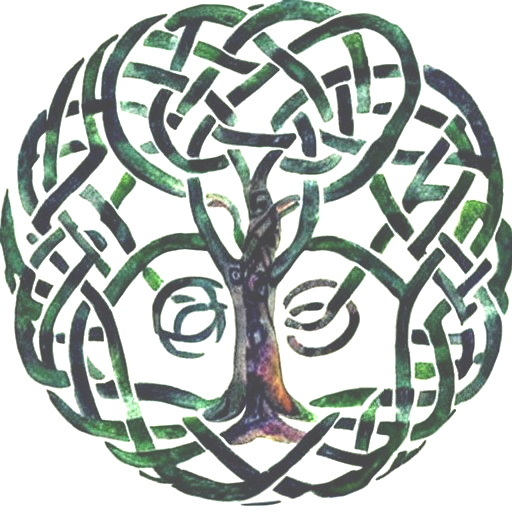
\includegraphics[height=11cm]{images/tree-cover} 
\end{center}
\thispagestyle{empty}
\newpage
\thispagestyle{empty}  % to not have a page# here

\selectlanguage{russian}
% \backgroundsetup{scale=1,opacity=1,angle=0,contents={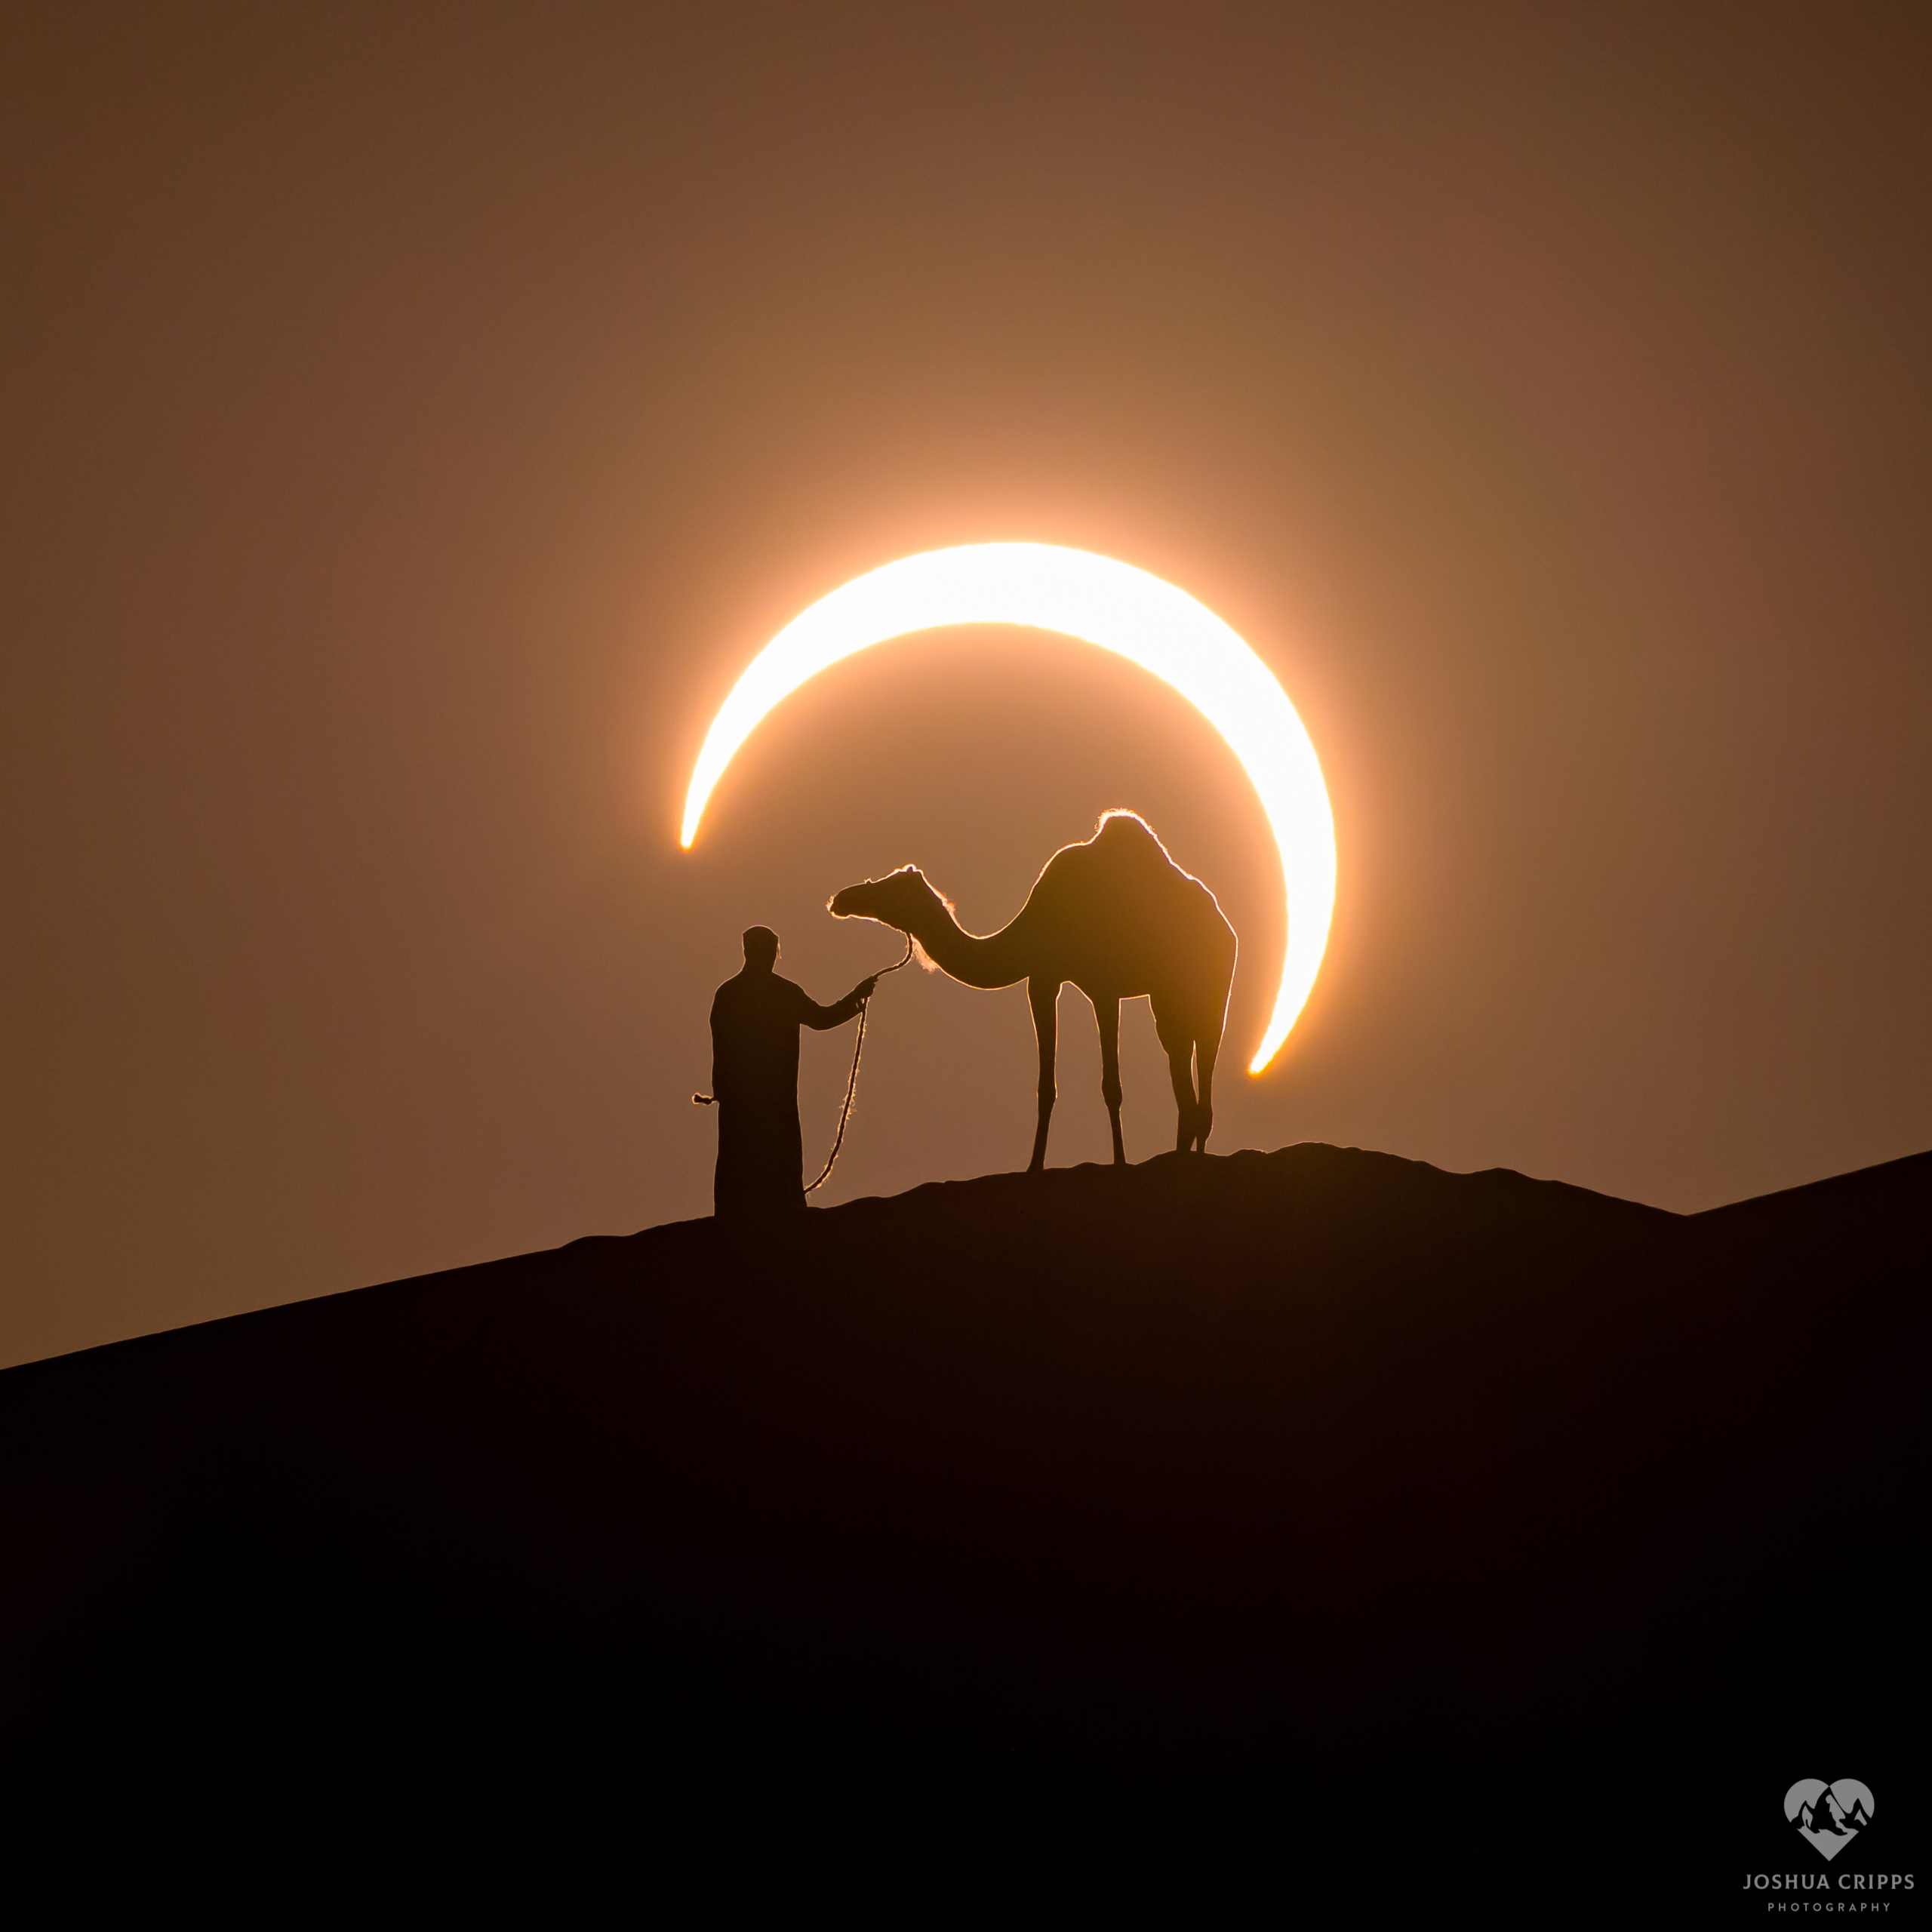
\includegraphics[width=\paperwidth,height=\paperheight]{eclipse.jpg}}}

\clearpage
% uncomment the line below to hide page number 
% \thispagestyle{empty}
\hfill

\backgroundsetup{scale = 1, angle = 0, opacity = 0.02, contents = {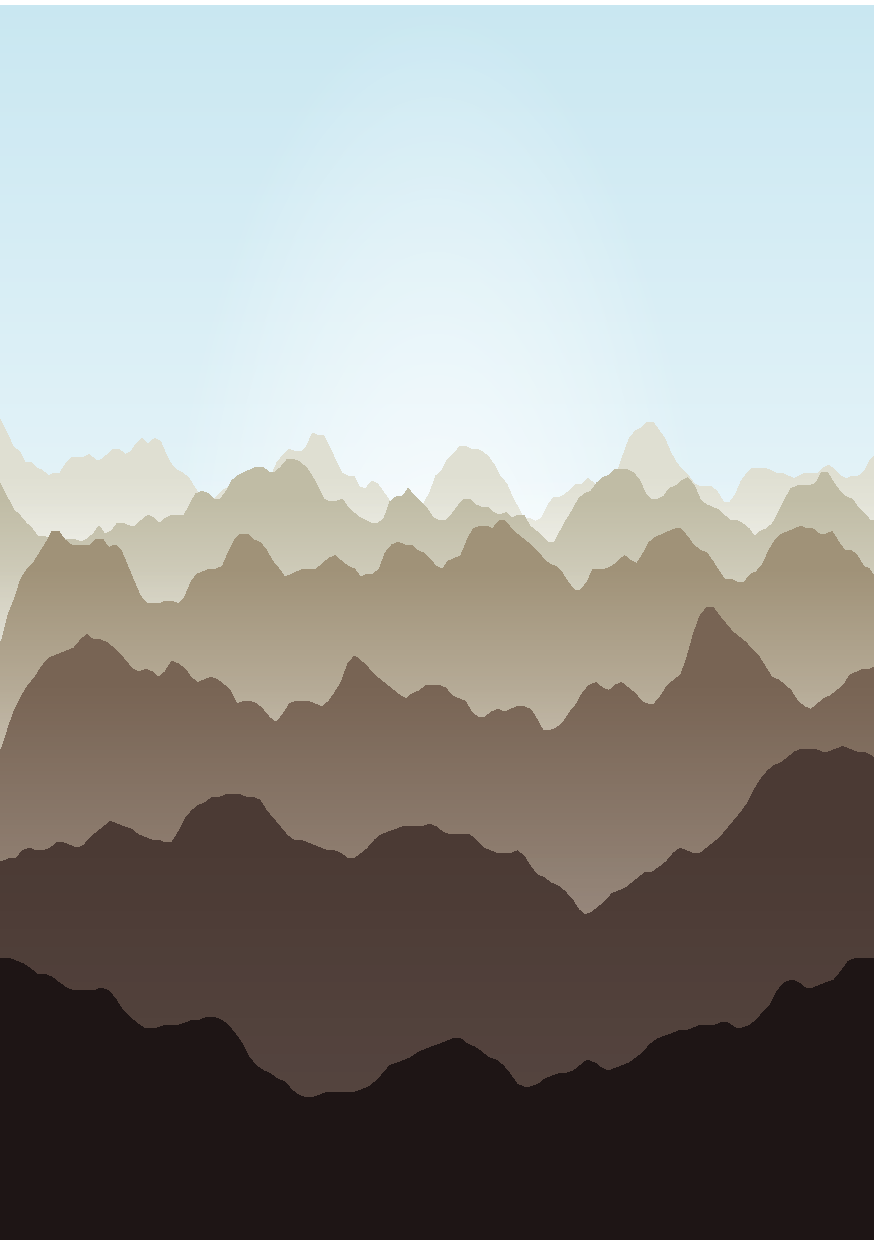
\includegraphics[width = \paperwidth, height = \paperheight] {images/mountains.pdf}}}
\BgThispage

\newpage

\addto\captionsrussian{ 
}
% so the table of contents itself is not shown in the table of contents
\begin{KeepFromToc}
  \tableofcontents
\end{KeepFromToc}

\backgroundsetup{scale = 1, angle = 0, opacity = 0.45, contents = {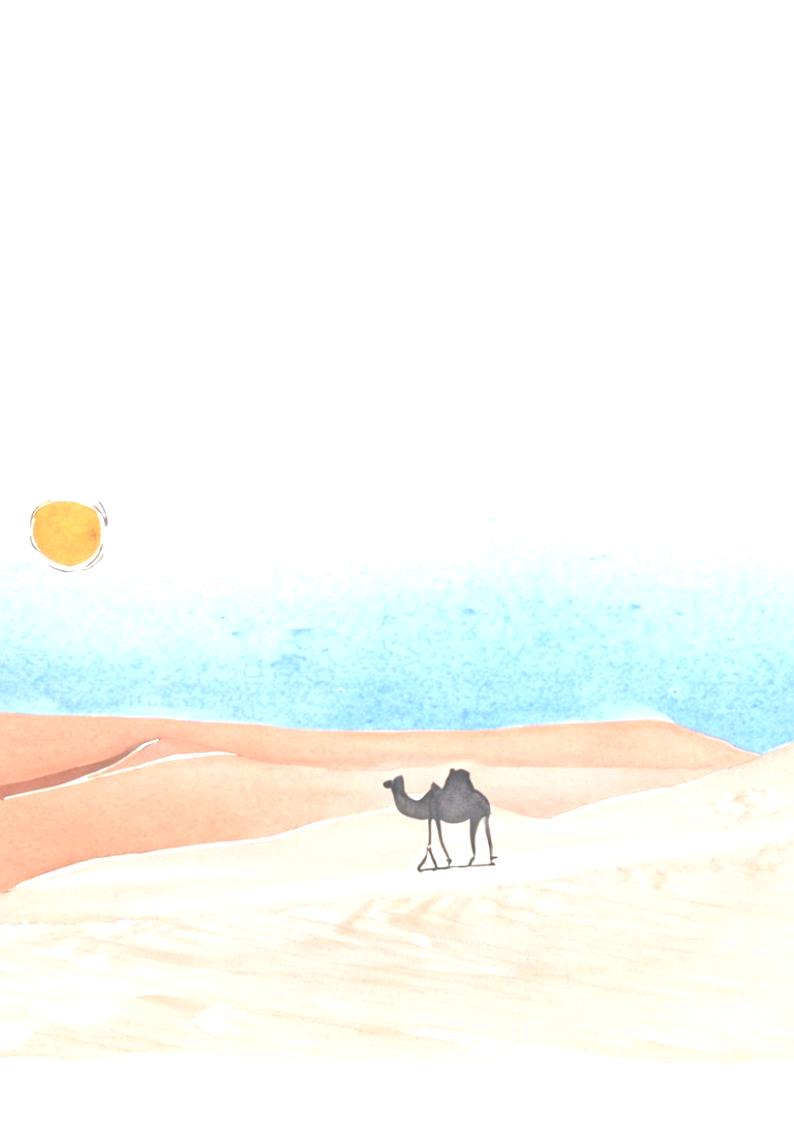
\includegraphics[width = \paperwidth, height = \paperheight] {images/camel}}}
\BgThispage


\thispagestyle{empty}  % hide page number
\newpage


\pagenumbering{arabic}  % so the second page begins with #1

% Show only the LEFT side of a landscape A4 drawing
\backgroundsetup{scale = 1, angle = 0, opacity = 0.05, contents = {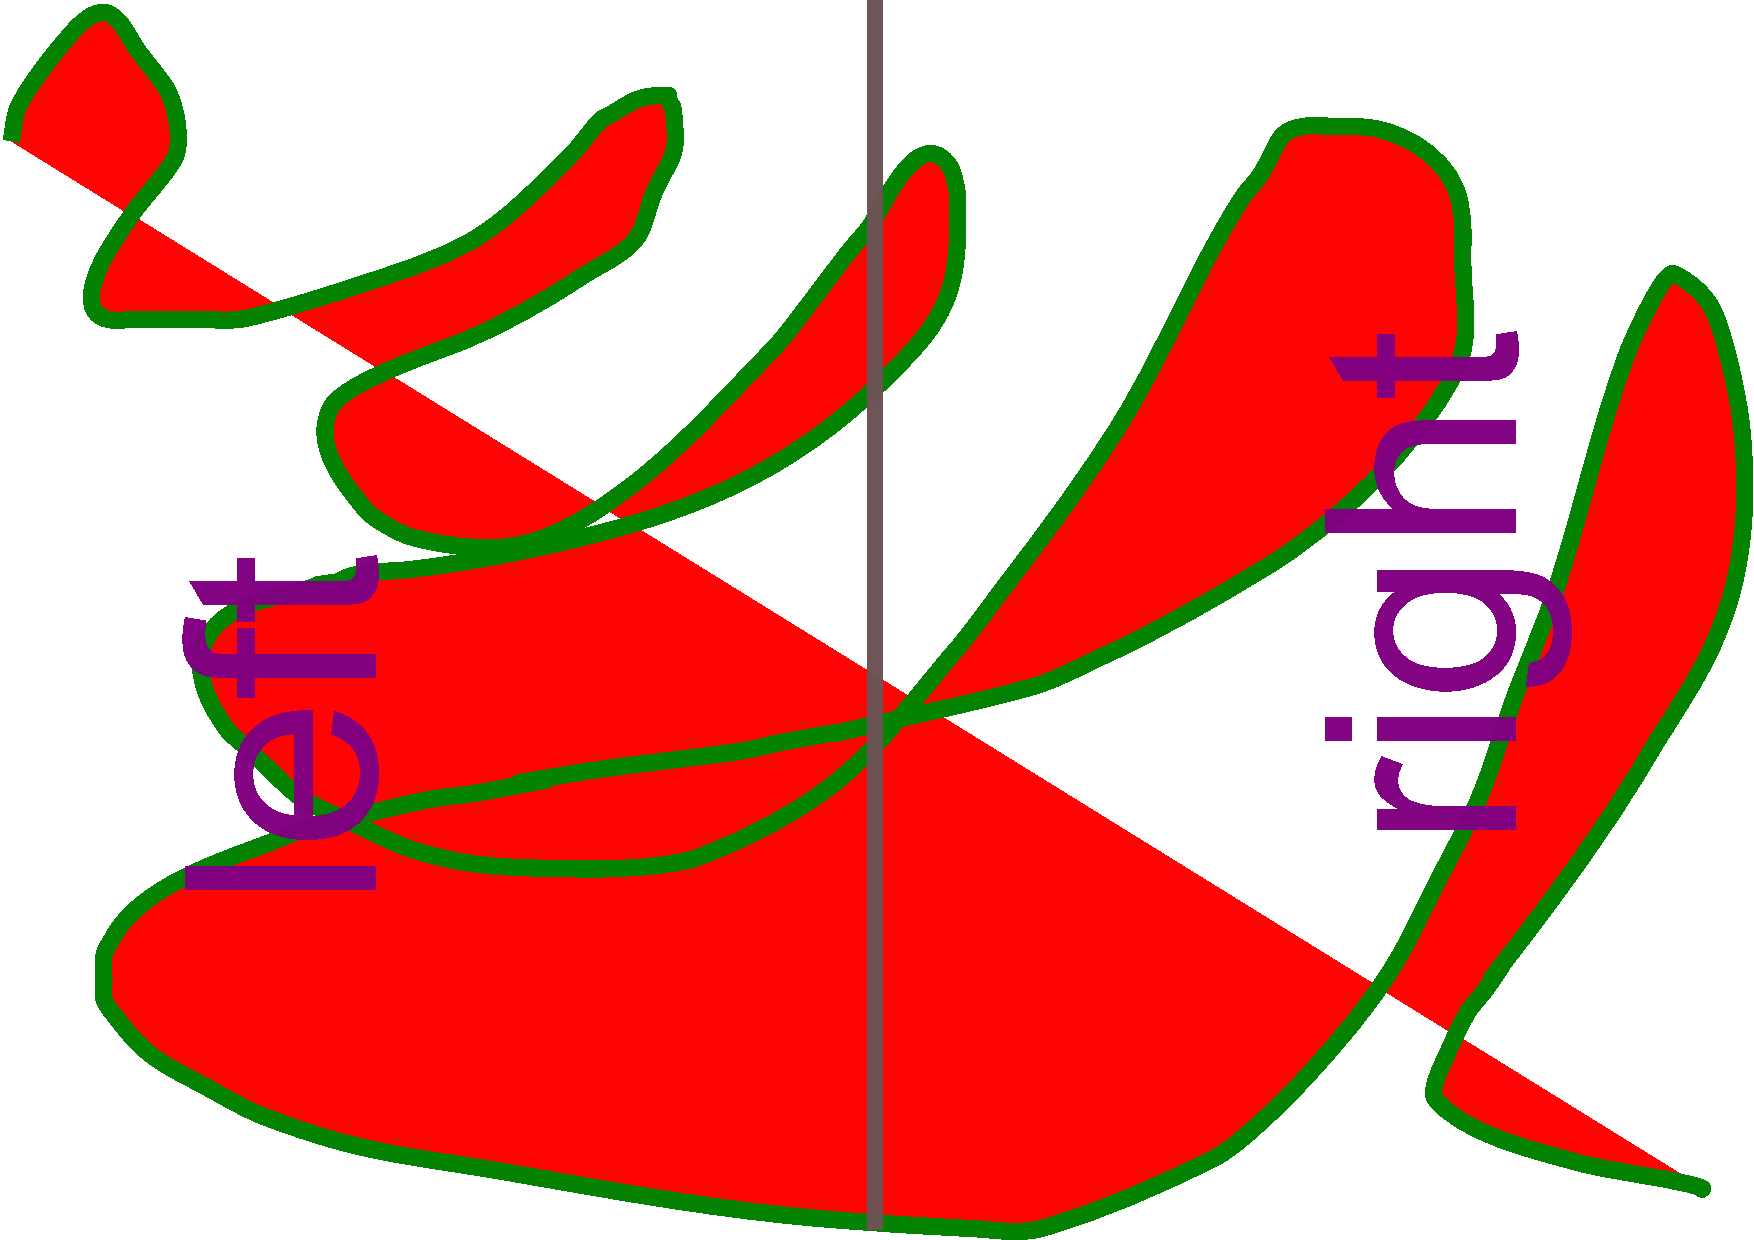
\includegraphics[width = \paperwidth, height = \paperheight,trim={0 0 148mm 0},clip] {images/spreadexperiment}}}
\BgThispage
% This is to move the poem to the right side, when printed
% as a booklet

\clearpage
% uncomment the line below to hide page number 
% \thispagestyle{empty}
\hfill
\clearpage

% Show only the RIGHT side of a landscape A4 drawing
\backgroundsetup{scale = 1, angle = 0, opacity = 0.05, contents = {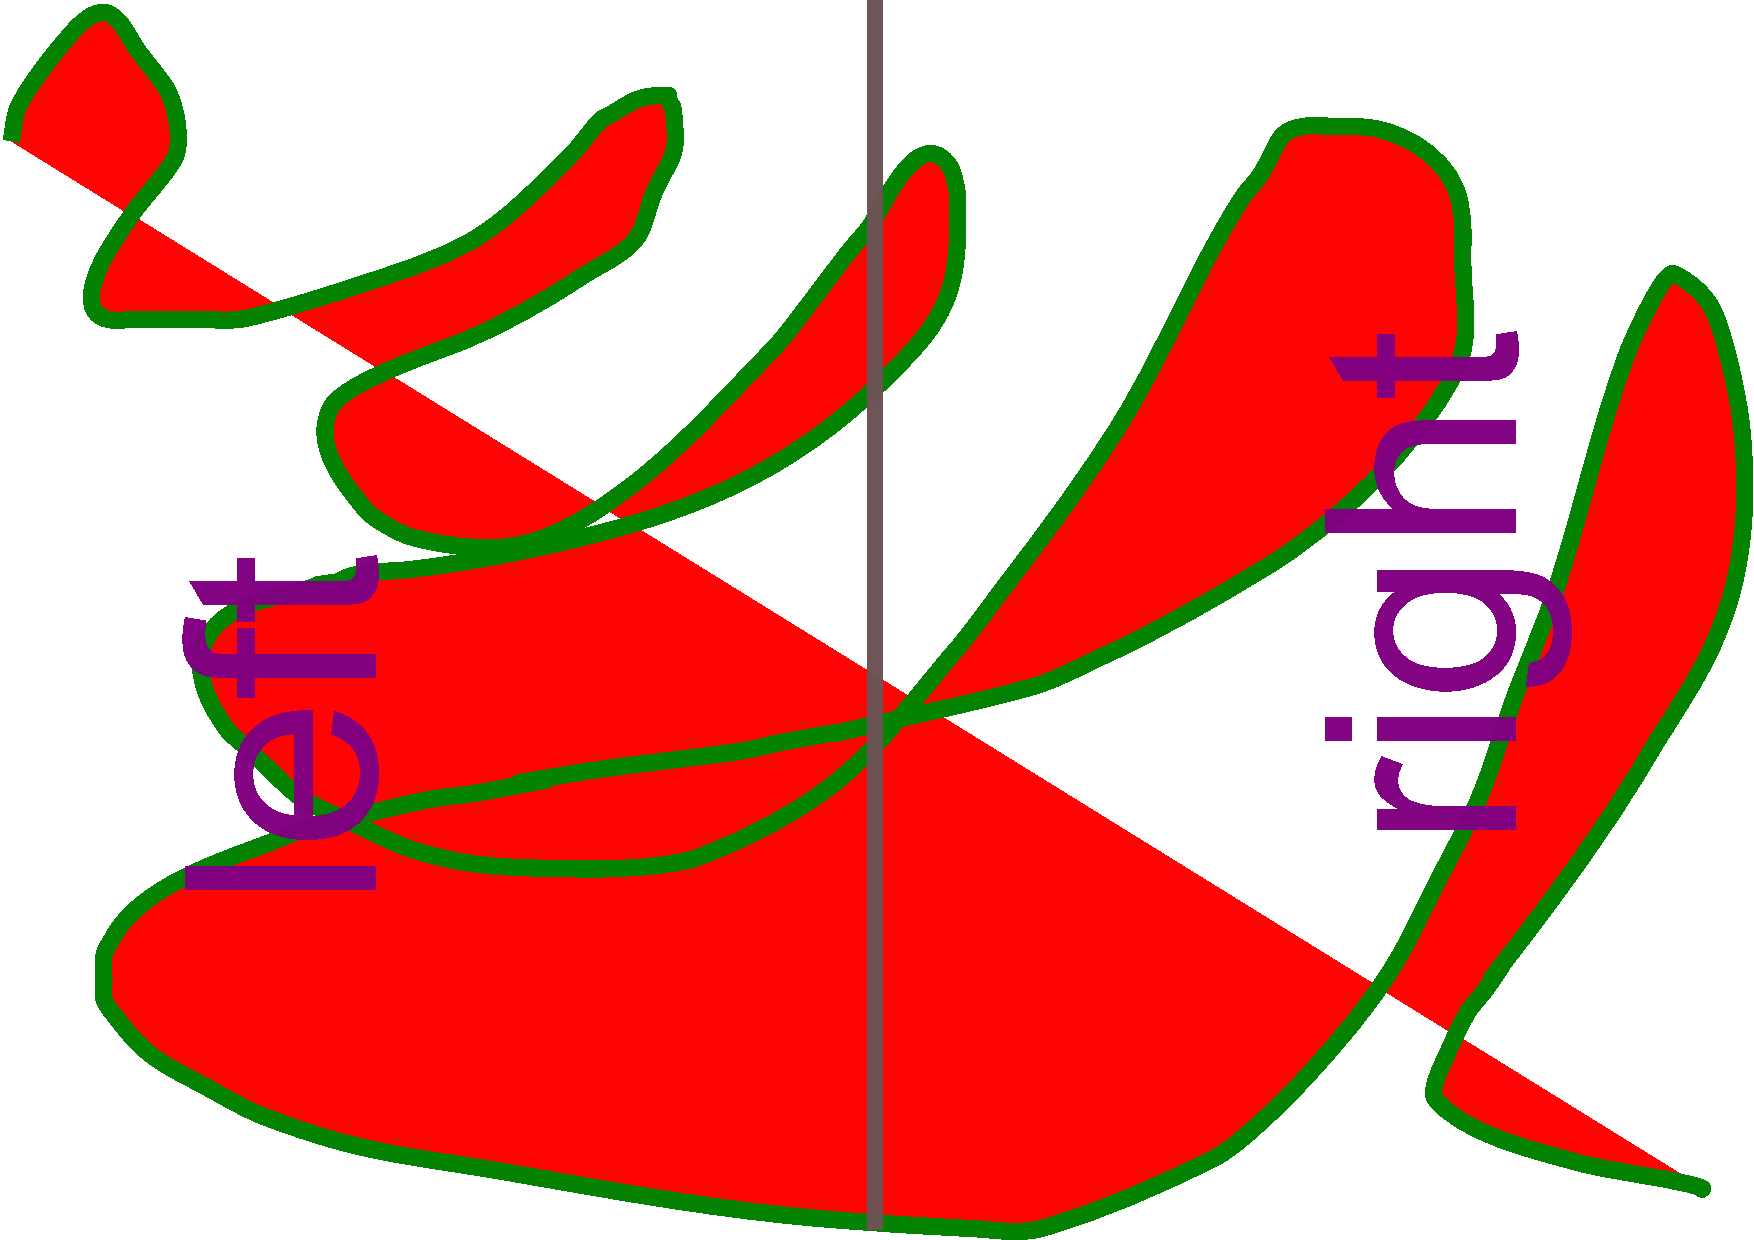
\includegraphics[width = \paperwidth, height = \paperheight,trim={148mm 0 0 0},clip] {images/spreadexperiment}}}
\BgThispage

\PlainPoemTitle
\PoemTitle{Харитон и хакатон}
\settowidth{\versewidth}{Серый кот - господин Мыцумото.}
\begin{verse}[\versewidth]
Жил-был добрый слон,\\
И звали его Харитон.
\end{verse}

\begin{verse}[\versewidth]
Прихватив клавиатуру под мышку,\\
по комнате шёл он вприпрыжку.\\
Хоботом, словно ракету,\\
подкинул он в воздух кассету\footnote{Кассету он получил от друга из Австралии.}.\\
А та, как диктует закон,\\
параболой --- в магнитофон!
\end{verse}

\begin{center}
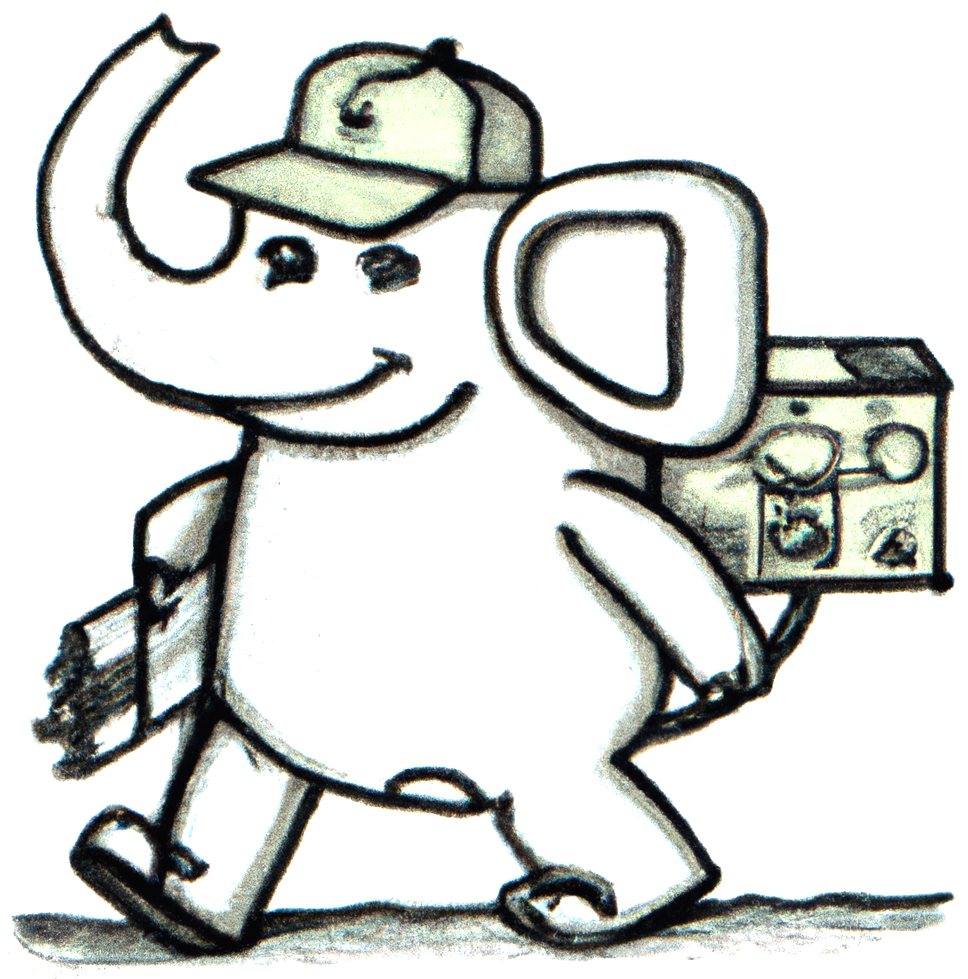
\includegraphics[height=11cm]{images/hariton.png} 
\end{center}
\newpage

\begin{verse}[\versewidth]
Летит и порхает как бабочка слон,\\
жужжит на плече его мáгнитофон,\\
ступеньки под весом скрипят и трещат --- \\
слона не легко на себе удержать!
\end{verse}

\begin{verse}[\versewidth]
И радость его не находит границы,\\
смеются в слоне даже микрочастицы!\\
Ведь знает, ведь знает,\\
наш слон, Харитон,\\
что путь приведёт его на Хакатон!
\end{verse}

\begin{verse}[\versewidth]
Он встретится там со своими друзьями,\\
с питоном, пингвином, гну, и с китами!\\
И вместе они порешают задачи,\\
чтоб мир вдруг стал лучше,\\
чтоб мир жил иначе!
\end{verse}

\begin{verse}[\versewidth]
Чтоб дети планеты могли без забот\\
глядеть в телескоп, в микроскоп --- круглый год!\\
Чтоб насмотревшись Вселенной красот,\\
достигнули в жизни новых высот.
\end{verse}

\newpage



\backgroundsetup{scale = 1, angle = 0, opacity = 0.9, contents = {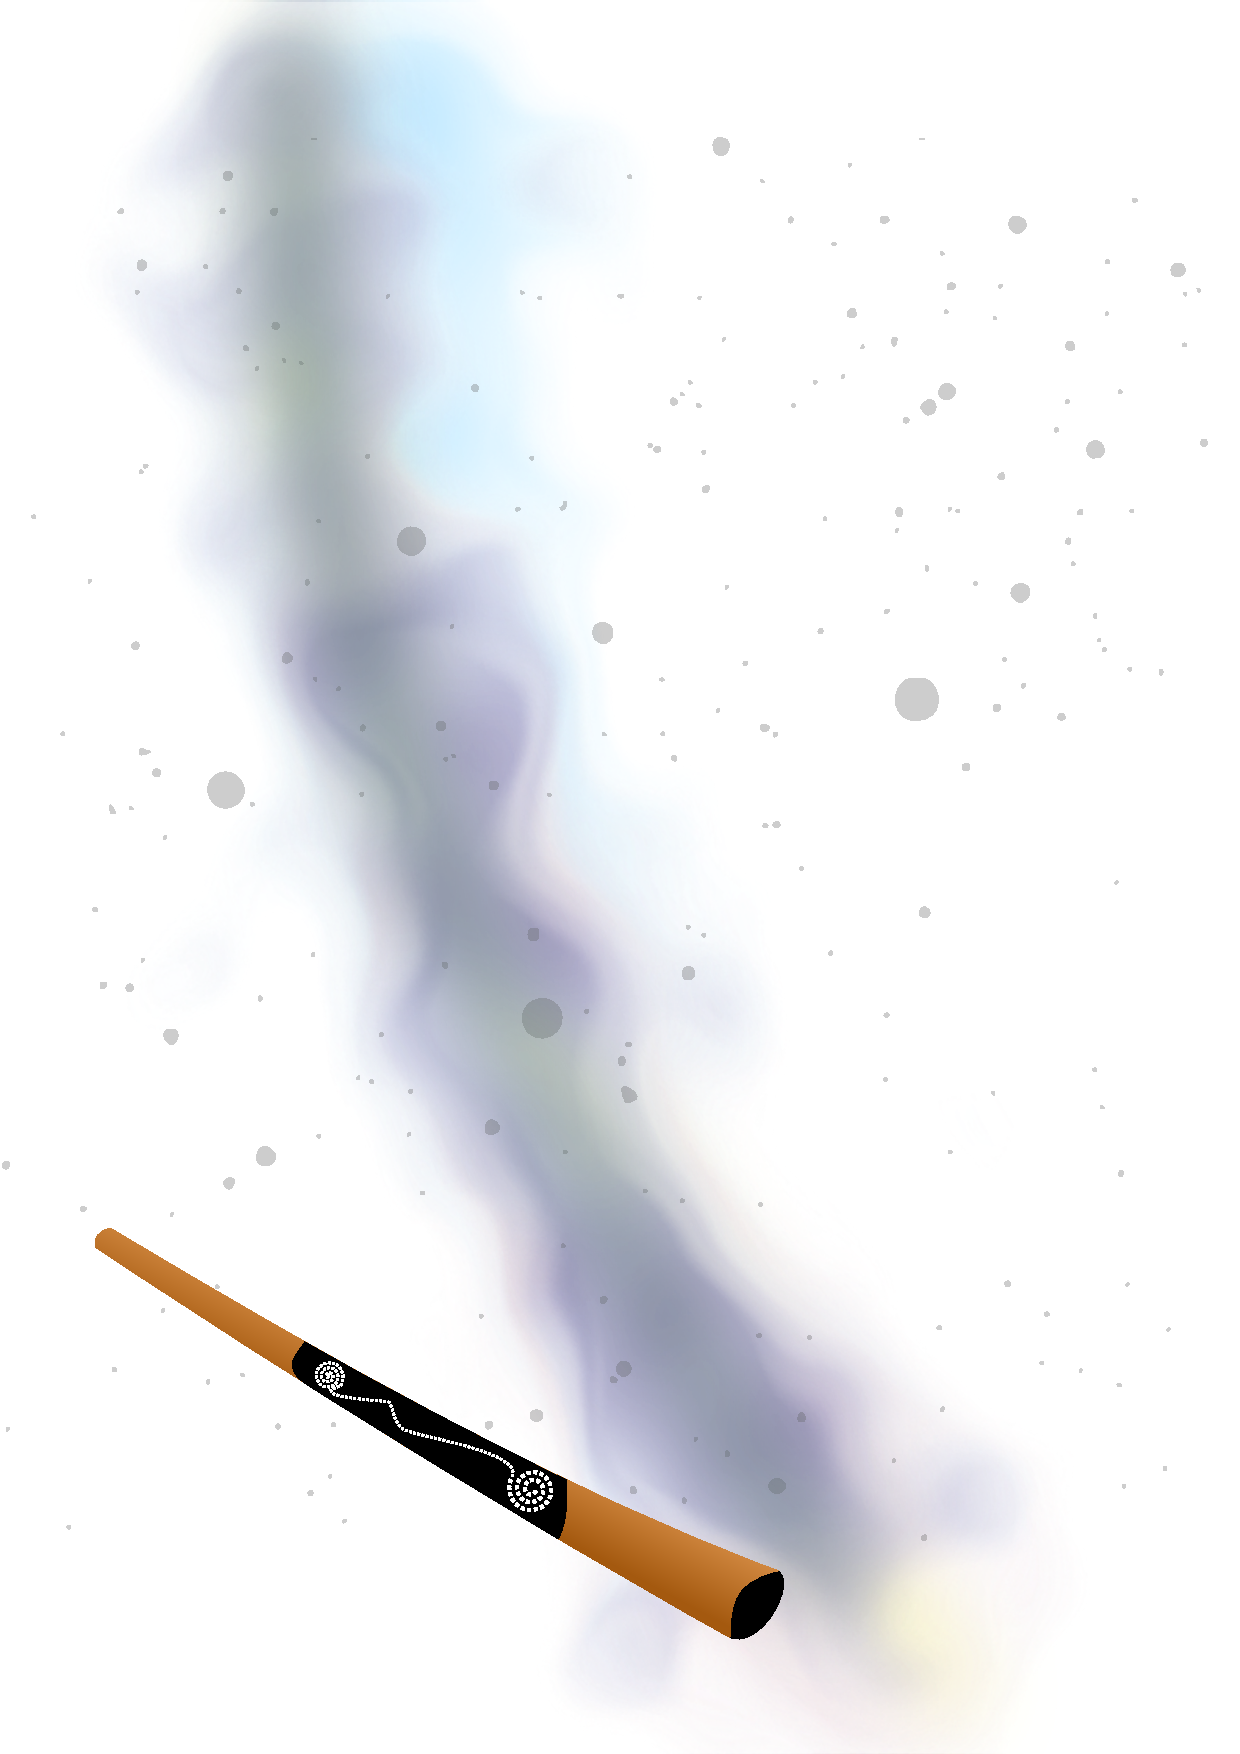
\includegraphics[width = \paperwidth, height = \paperheight] {images/night-sky}}}
\BgThispage

% \renewcommand{\poemtoc}{subsection}
% \PlainPoemTitle
\PoemTitle{Кенгуру у Улур\'{у}}
\settowidth{\versewidth}{Серый кот - господин Мыцумото.}
\begin{verse}[\versewidth]
Как-то раз у горы Улур\'{у}\\
собрались вомб\'{а}т, утконос и эм\'{у}.\\
Уселись они у костра, потеплее\\
и стали разглядывать звезды на небе.
\end{verse}
\label{milky-way}


\begin{verse}[\versewidth]
Одна звезда, две звезды, три, и четыре\ldots\\
зрачки разрастались всё шире и шире,\\
как только их счёт дошёл до пяти\\
их уши услышали чьи-то прыжки.
\end{verse}

\begin{verse}[\versewidth]
Это их друг --- артист кенгуру,\\
он любит ночами ходить к Улур\'{у}.\\
Приблизившись к свету, увидев вомбата,\\
он крикнул \emph{``я рад нашей встрече, ребята!\\
Можно я с вами чуть-чуть посижу?''}\\
\emph{``Конечно! Садись!''} в хор сказали ему.
\end{verse}

\begin{verse}[\versewidth]
Присев у огня, артист кенгуру\\
Вынул из сумочки диджериду.\\
Вздохнув глубоко, посмотрев на луну,\\
махая хвостом он сказал \emph{``счас спою!''}
\end{verse}

% \vspace{1cm}
% \begin{center}
% 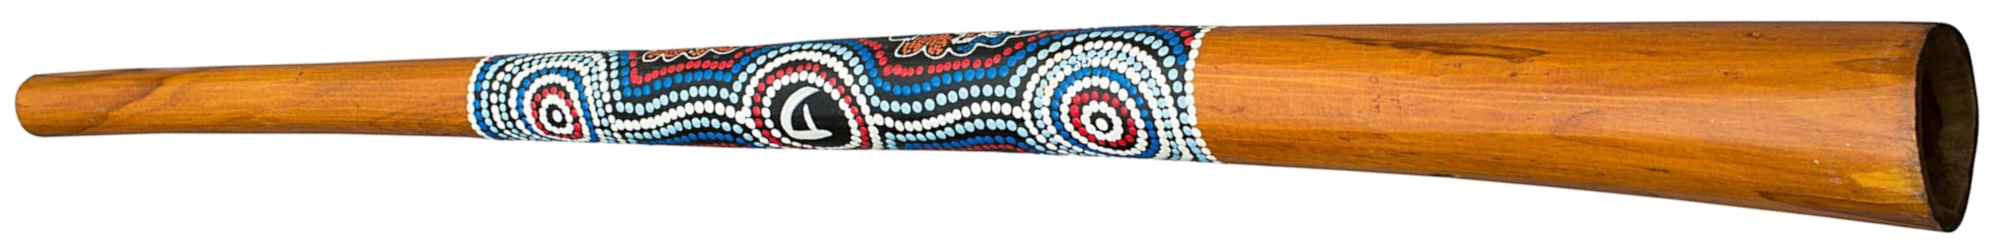
\includegraphics[width=0.6\paperwidth]{images/didgeridoo} 
% \end{center}



\newpage
\hfill

\backgroundsetup{scale = 1, angle = 0, opacity = 0.45, contents = {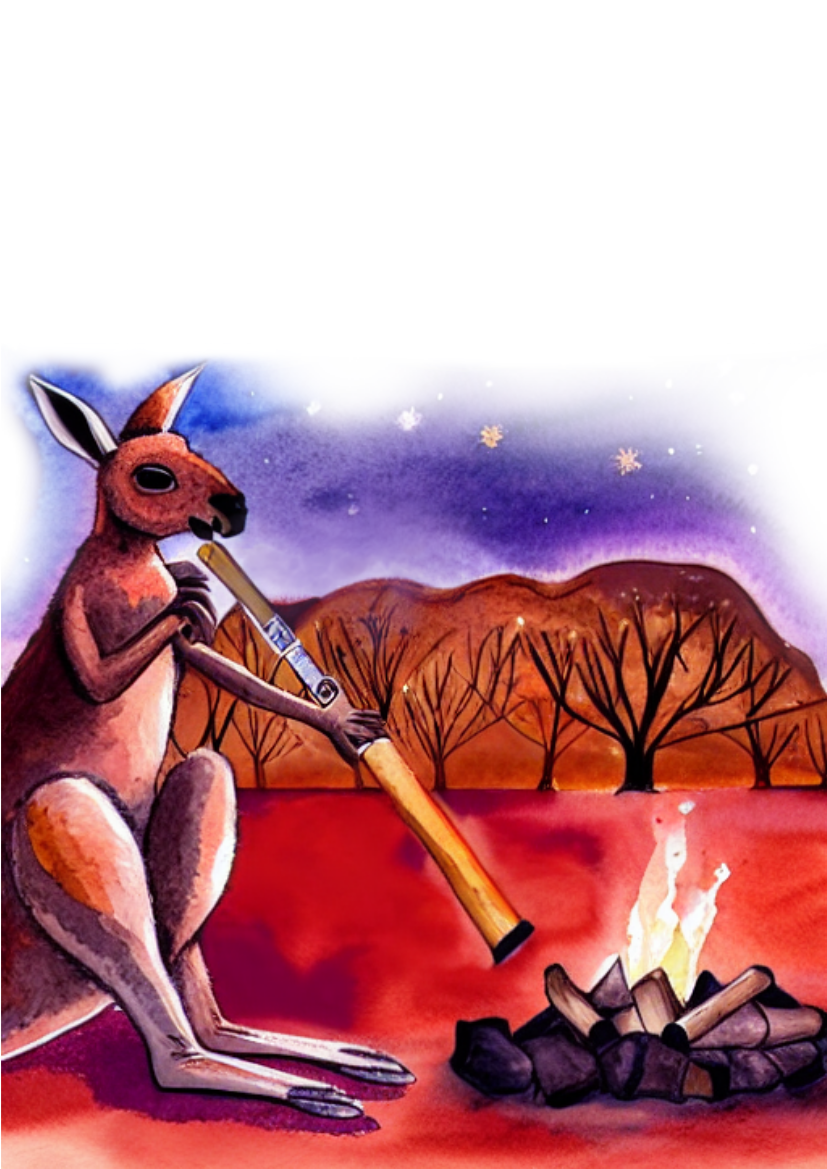
\includegraphics[width = \paperwidth, height = \paperheight] {images/kangaroo-final}}}
\BgThispage
% \newpage


% \fancybreak{* * *}

\begin{verse}[\versewidth]
Вздулись внезапно вокруг паутины\\
гул вырастал в австралийской пустыне.\\
Вууу--{\largeдууу}--{\Largeбууу}--{\LARGEдууу!}\\
Всё громче и громче диджериду!\\
\emph{``{\LargeВууу}--{\largeдууу}--буу--{\smallдууууу!}''}\\
Эхом ответила вслед Улур\'{у}.
\end{verse}
\newpage



\backgroundsetup{scale = 1, angle = 0, opacity = 0.7, contents = {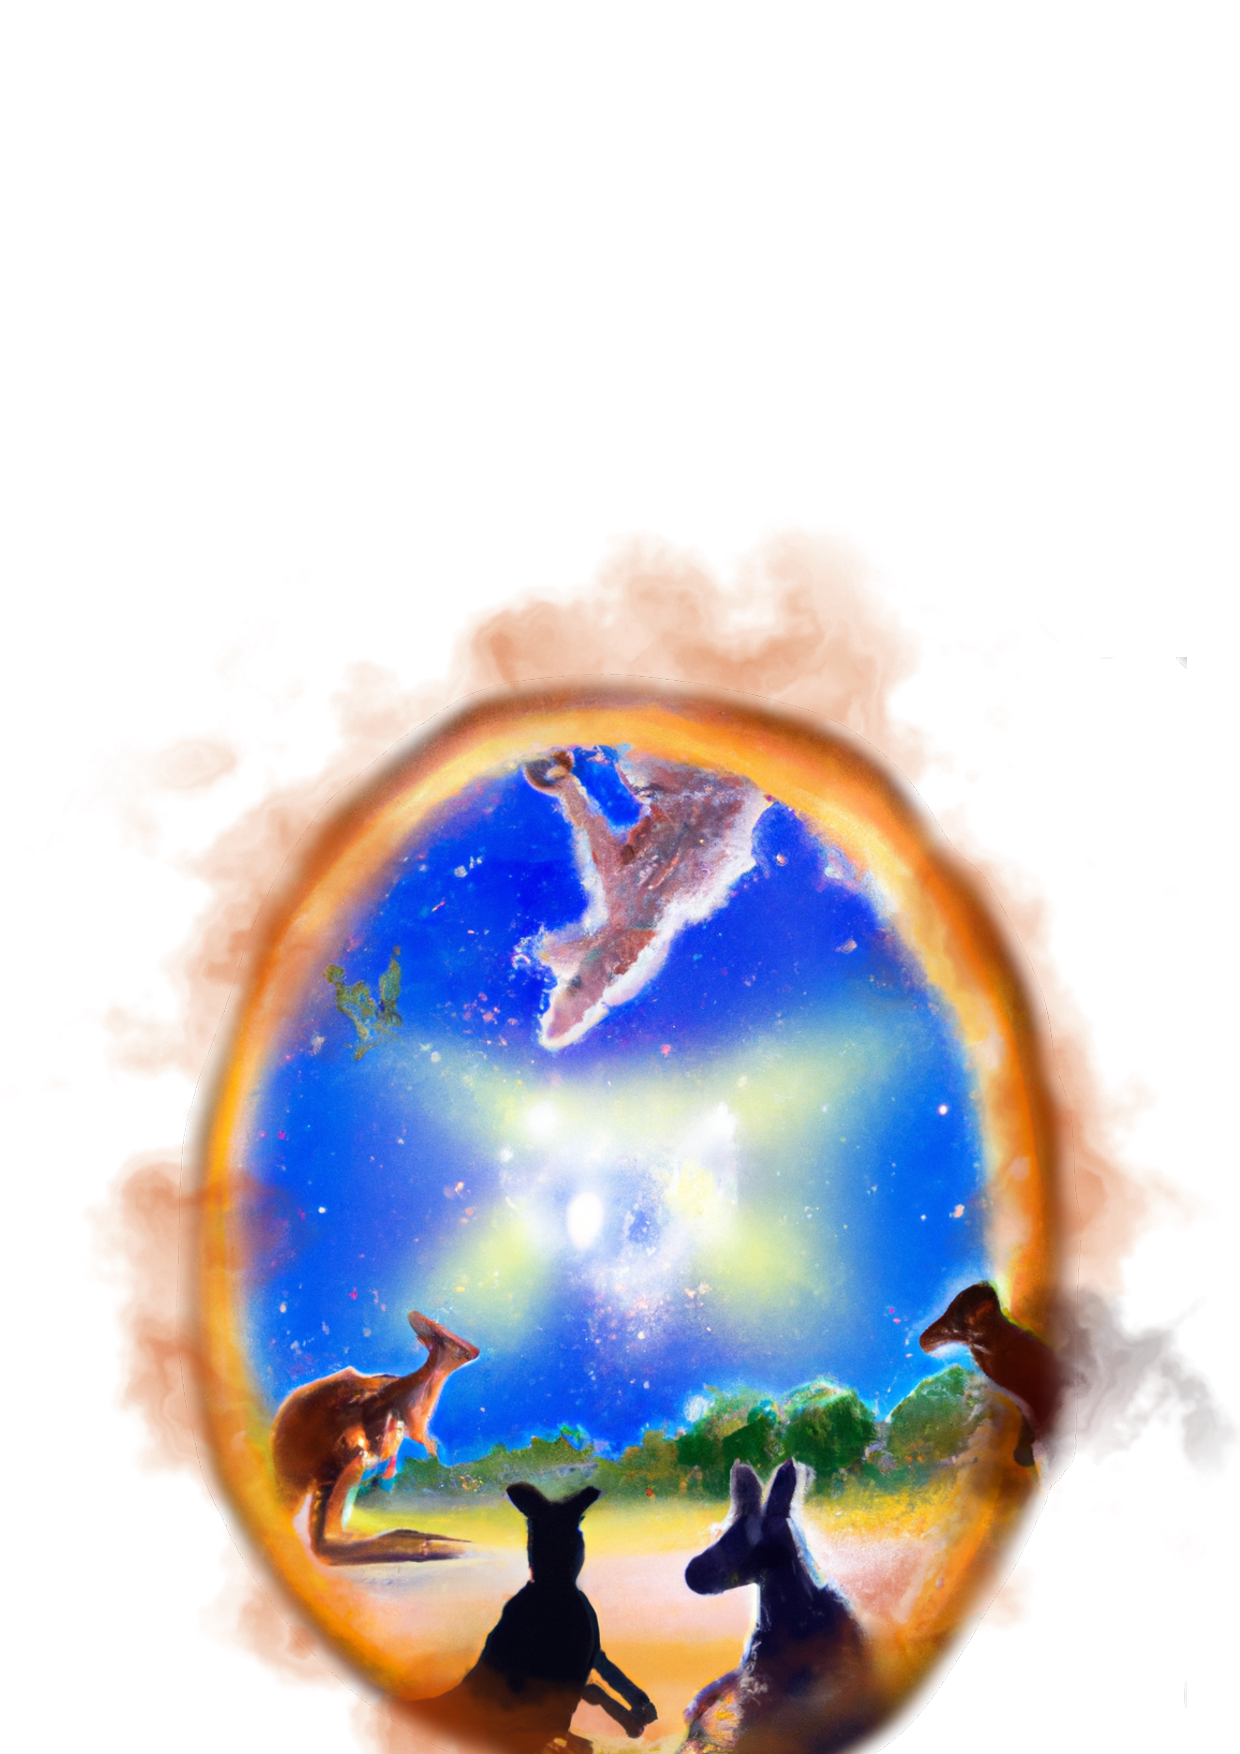
\includegraphics[width = \paperwidth, height = \paperheight] {images/portal}}}
\BgThispage



\begin{verse}[\versewidth]
Такт отбивая правой ногой\\
дверь распахнул кенгуру в мир иной!\\
Звук можно чувствовать клеткой грудной,\\
эм\'{у} кивает в ритм головой.
\end{verse}

% \vspace{4cm}
\begin{verse}[\versewidth]
Все они вдруг от земли оторвались\\
и среди звёзд через миг оказались!\\
Волна их несёт по теченью Пути,\\
ночь разукрасилась, стала цвести!
\end{verse}

\newpage

\begin{verse}[\versewidth]
Вокруг облака бесконечно, и снова,\\
точкой становятся, затем и сверхновой.\\
Время летит то вперёд, то назад,\\
утконос ничего не может понять!
\end{verse}

\backgroundsetup{scale = 1, angle = 0, opacity = 0.3, contents = {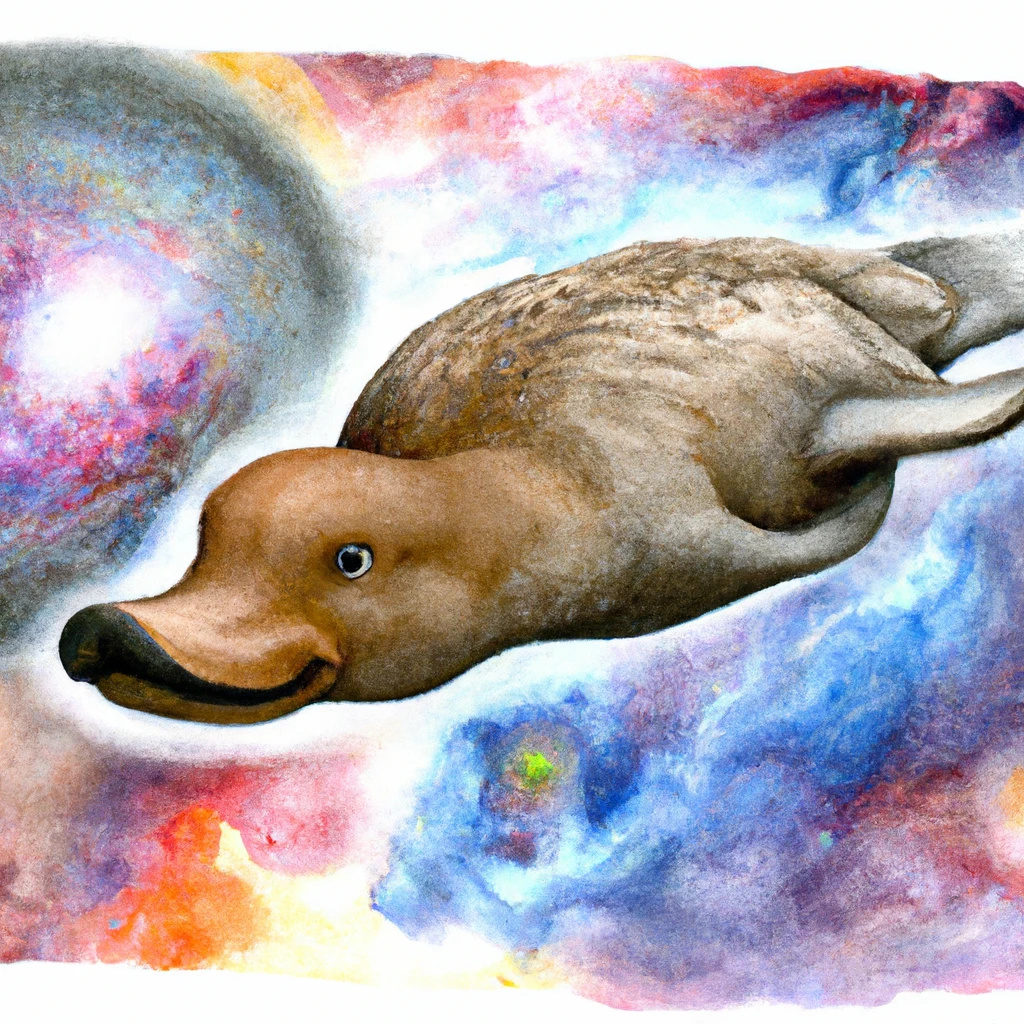
\includegraphics[width = \paperwidth, height = \paperheight] {images/dazed-platypus}}}
\BgThispage

% \begin{center}
% 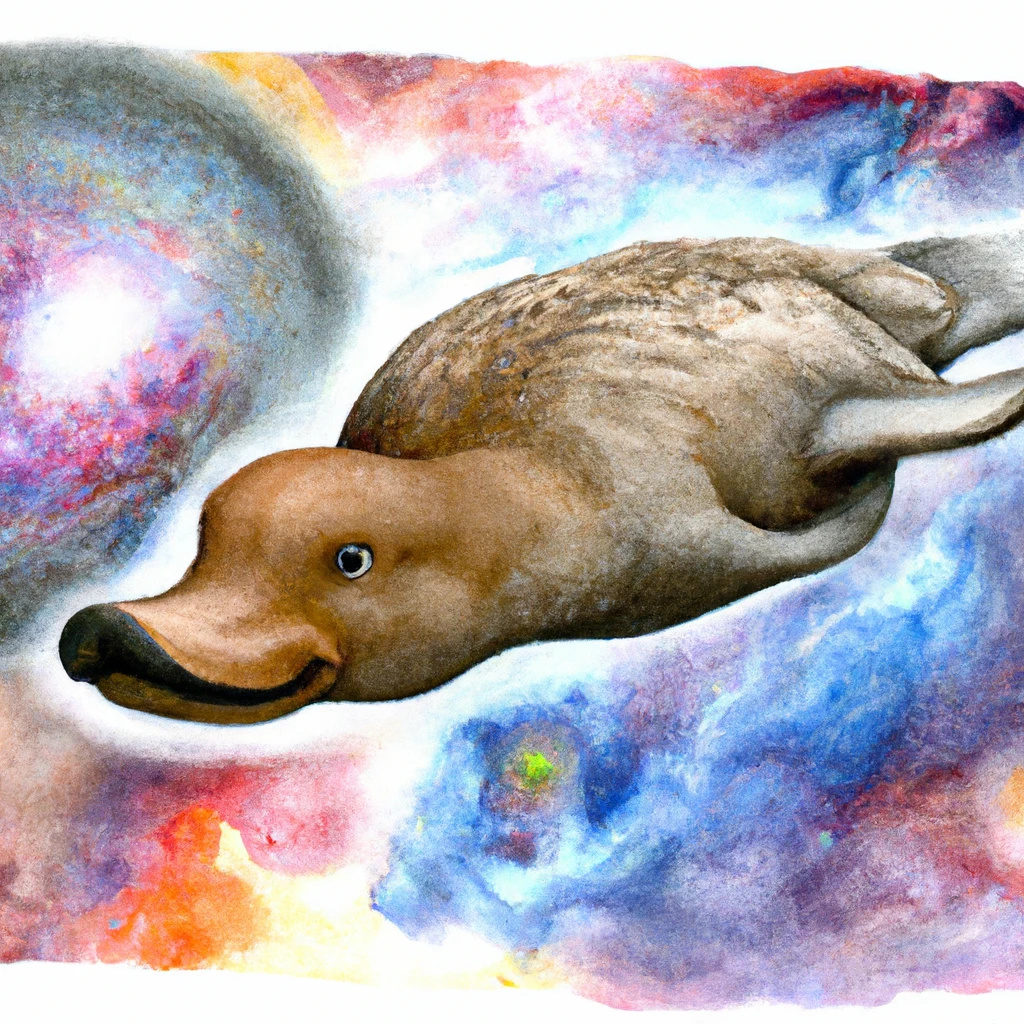
\includegraphics[width=\paperwidth]{images/dazed-platypus.jpg} 
% \end{center}

\vspace{12cm}
\begin{verse}[\versewidth]
Диджериду продолжает гудеть,\\
утконосу от радости хочется петь!\\
Космос раскрылся как цветок на ладони,\\
ритм всё пространство собою заполнил.\\
Нету начала, и нету конца,\\
эта мелодия везде и всегда!
\end{verse}
\newpage

% \fancybreak{* * *}

\begin{verse}[\versewidth]
Солнце вернулось из-за горизонта,\\
гора Улур\'{у} загорелась как охра.\\
Пустыня ожила, и ветер задул,\\
а наш кенгурёнок наконец-то уснул!
\end{verse}

\label{uluru}
\backgroundsetup{scale = 1, angle = 0, opacity = 0.6, contents = {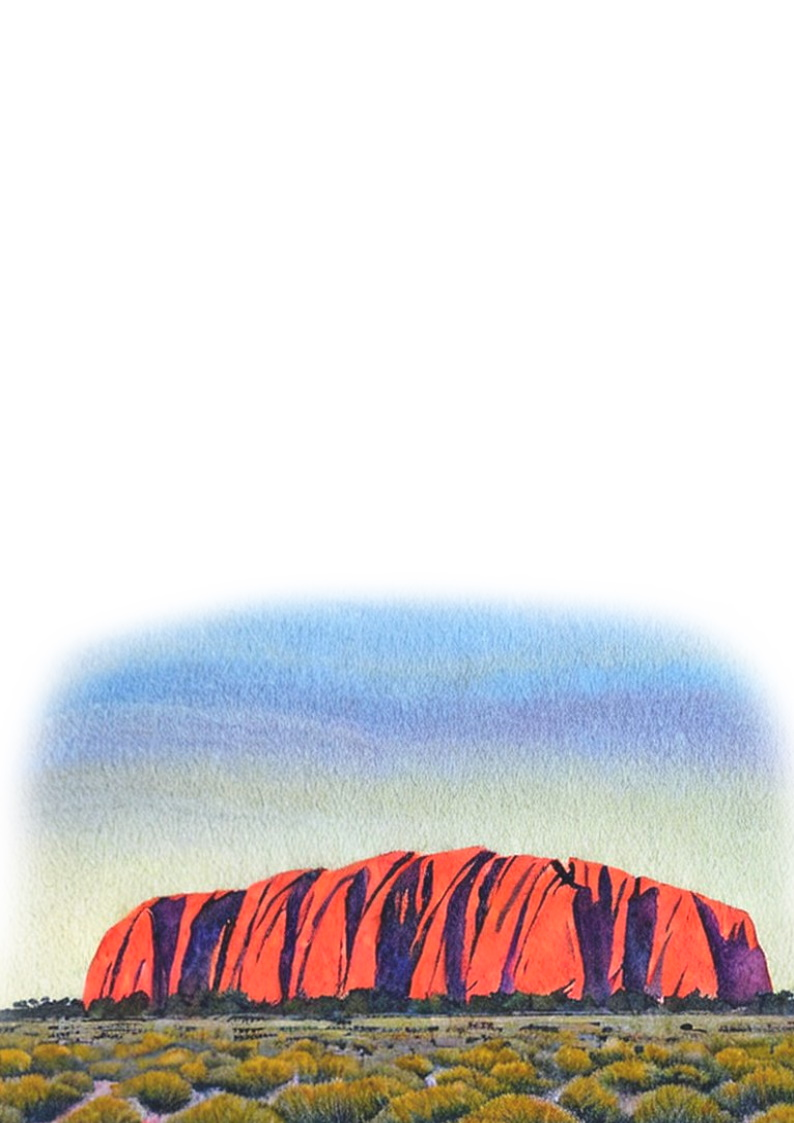
\includegraphics[width = \paperwidth, height = \paperheight] {images/uluru}}}
\BgThispage

\newpage



\PlainPoemTitle
\PoemTitle{Мыцумото из Киото}
% \settowidth{\versewidth}{Серый кот - господин Мыцумото.}
\begin{verse}[\versewidth]
Жил был в префектуре Киото\\
рыжий кот --- господин Мыцумото.\\
Прыгнув однажды в окно, \\
хвостом он задел кимоно. 
\end{verse}

\begin{verse}[\versewidth]
Шелком шурша\\
вещь как листик летала,\\
вазу задела --- ваза упала;\\
к чашке притронулась ---\\
чашка разлилась;\\
лампа на тумбочке\\
вдруг заискрилась.
\end{verse}

\begin{verse}[\versewidth]
Ваза разбилась,\\
разлетелись кусочки, \\
на полу оказались \\
из вазы цветочки. \\
\end{verse}

\backgroundsetup{scale = 1, angle = 0, opacity = 0.25, contents = {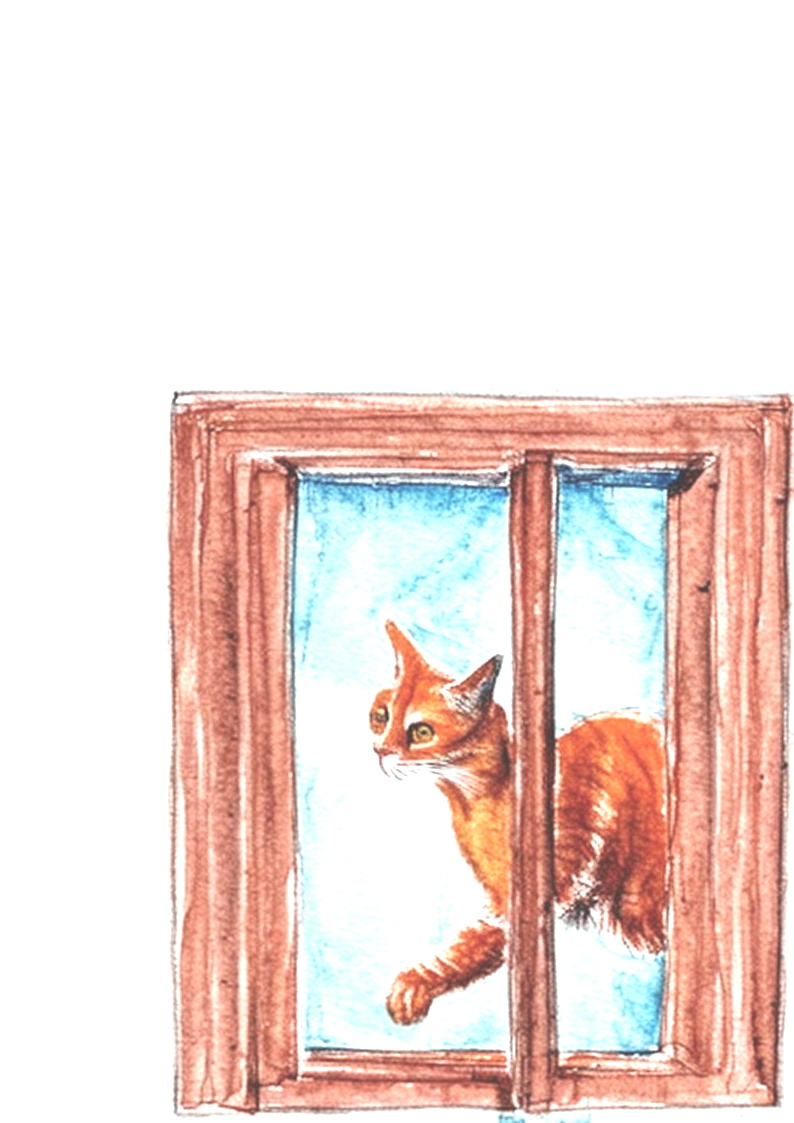
\includegraphics[width = \paperwidth, height = \paperheight] {images/cat-window}}}
\BgThispage


\clearpage
\backgroundsetup{scale = 1, angle = 0, opacity = 0.45, contents = {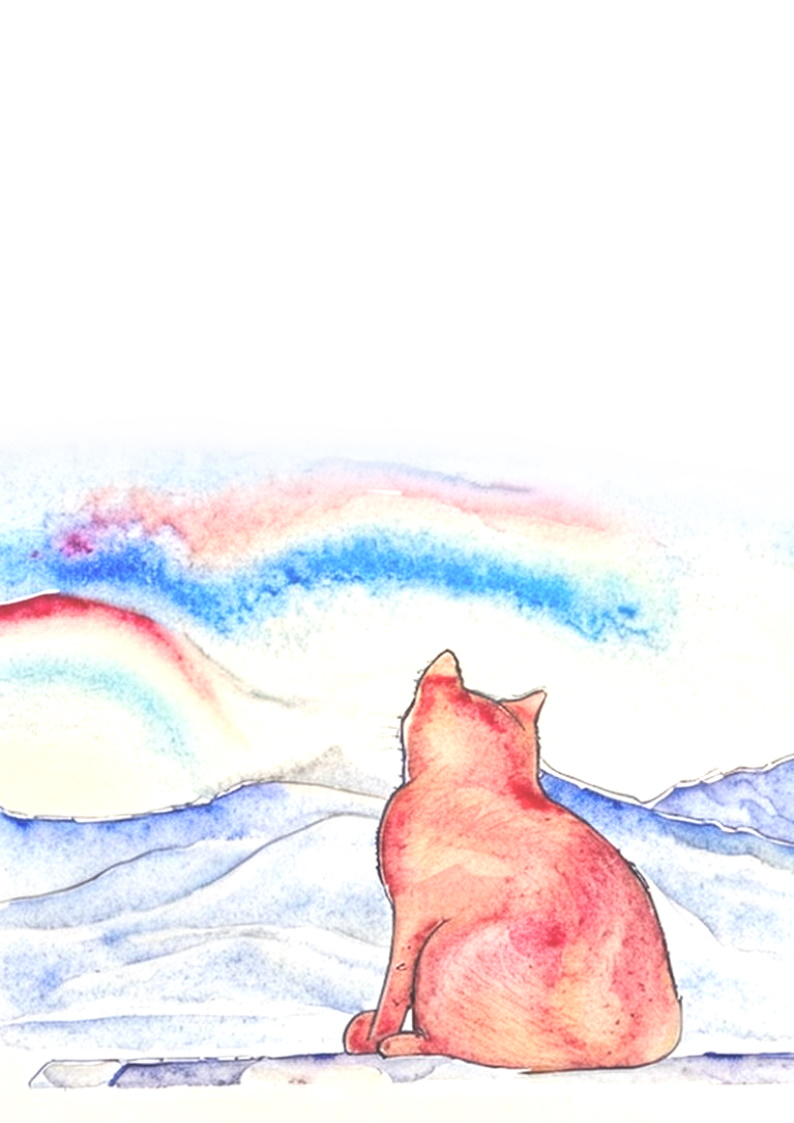
\includegraphics[width = \paperwidth, height = \paperheight] {images/cat}}}
\BgThispage

\fancybreak{* * *}

\begin{verse}[\versewidth]
На шерсти почувствовав солнца лучи \\
смотрел Мыцумото на горы вдали. \\
\emph{``Ах, как прекрасно день начался! \\
Так приятно купаться в рассвета лучах!''}
\end{verse}

\begin{verse}[\versewidth]
В небесах облака словно множество линий \\
градиент переходит из красного в синий, \\
птицы запели, раскрылись цветы, \\
не осталось ни следа от темноты. 
\end{verse}

\begin{verse}[\versewidth]
На коврике сидя, господин Мыцумото\\ 
забыл о работе, забыл о заботах\ldots \\
он слился с природой, \\
растворил в ней свой ум,\\ 
всё вдруг затихло, исчез всякий шум\ldots 
\end{verse}

\clearpage
\fancybreak{* * *}

\begin{verse}[\versewidth]
Вернувшись обратно, запрыгнув в окно, \\
Мыцумото заметил что что-то не то. \\
Он тихо поднял и сложил кимоно. 
\end{verse}

\begin{verse}[\versewidth]
Он лапой собрал на полу лепесточки, \\
временно в банку поставил цветочки,\\ 
лампу протёр, починил выключатель, \\
чашку поднял, промяукав \emph{``что дальше?''} 
\end{verse}

\begin{verse}[\versewidth]
А дальше он вазы нашёл все кусочки \\
и клей-порошок он достал из мешочка,\\
собрал воедино, как паззл осколки, \\
уж очень любил он\ldots ~головоломки!
\end{verse}

\begin{verse}[\versewidth]
Трещины кисточка лаком ласкает, \\
керамику в жизненный путь возвращает. \\
на прежнее место цветочки вернулись\\ 
и к солнцу опять лепестки повернулись.
\end{verse}

\begin{verse}[\versewidth]
Стала теперь наша ваза сильнее, \\
господин Мыцумото --- стал чуть мудрее.
\end{verse}

\begin{center}
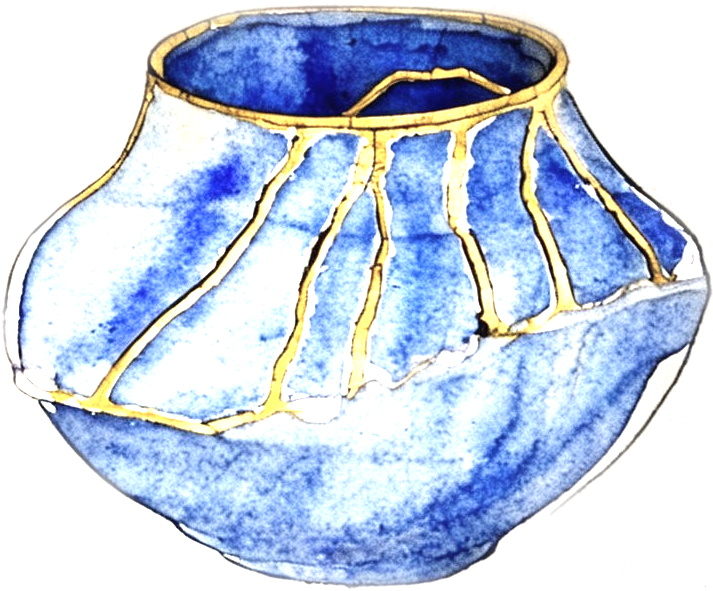
\includegraphics[height=6cm]{images/vase} 
\end{center}
\newpage




\PlainPoemTitle
\PoemTitle{Может быть}
\vspace{-7mm}
\begin{center}\small{\textit{(по мотивам китайской сказки)}}\end{center}

\begin{verse}[\versewidth]
Жил-был в провинции Хубэй \\
да на ферме усердно работал, \\
Лао Вэнг ---  любимец детей, \\
с тремя сыновьями и дочкой. \\
\end{verse}

\begin{verse}[\versewidth]
Была у них лошадь с белою гривой, \\
была она умной, доброй, игривой\ldots \\
Любила лошадка по ферме скакать, \\
воду носить, да тележку таскать. \\
\end{verse}

\begin{verse}[\versewidth]
Утром, однажды, заметили все ---  \\
что стойло пустует, и лошади нет! \\
Засуетились люди в селе ---  \\
лошадь искали, искали везде\ldots \\
За холмами, в лесу, и вниз по реке\ldots \\
Но след от лошадки не найден нигде. \\
\end{verse}

\begin{verse}[\versewidth]
И сказали тогда все в селе: \\
\emph{``Вот горе! Вот невезенье! \\
Ах, великая беда! \\
Не повезло старине Лао Вэнгу, \\
ох и тяжелая эта судьба\ldots''} \\
\end{verse}

\begin{verse}[\versewidth]
Лао подумал, дал печали остыть, \\
помолчал, и сказал \emph{``может быть\ldots''} \\
\end{verse}

\begin{verse}[\versewidth]
Прошел день. \\
Прошло два. \\
Ночь накрыла село. \\
На небо явилась луна. \\
\end{verse}

\begin{verse}[\versewidth]
Всех разбудил шум копыт! \\
Неужели наступает орда?!?! \\
\end{verse}

\begin{verse}[\versewidth]
Это лошадка вернулась в село, \\
но вернулась она не одна! \\
Семь лошадей привела за собой: \\
шесть кобыл и коня! \\
\end{verse}

\begin{verse}[\versewidth]
Дикие звери, здоровые звери, \\
гривы как из серебра! \\
К Лао на ферму как ветер примчались, \\
и машут хвостами то туда, то сюда\ldots \\
\end{verse}

\begin{verse}[\versewidth]
\emph{``Вот повезло! Вот это удача! \\
Ну и везёт же тебе, старина! \\
Получил ты от жизни огромный подарок, \\
ах, вот это судьба!''} \\
\end{verse}

\begin{verse}[\versewidth]
Лао подумал, дал веселью остыть, \\
помолчал, и сказал \emph{``может быть\ldots''} \\
\end{verse}

\begin{verse}[\versewidth]
День спустя, все решили --- настала пора \\
узду натянуть на коня. \\
\end{verse}

\begin{verse}[\versewidth]
Старший сын собрал храбрость, \\
запрыгнул, схватившись за гриву. \\
Но конь несогласен с решением был, \\
уж очень свободу любил он! \\
\end{verse}

\begin{verse}[\versewidth]
ии{\Largeии}{\LARGEии}-{\hugeха!!!} То влево, то вправо! \\
Хрипит и кричит он как вихрь! \\
ии{\Largeии}{\LARGEии}-{\hugeхо!!!} То вперёд, то назад! \\
Не хочет нести он чужих! \\
\end{verse}

\begin{verse}[\versewidth]
Парень вцепился силой троих, \\
но конь не боится приёмов ручных! \\
Вдруг он затих. Собрал сил неземных,  \\
всадника скинул, сбив четверых! \\
\end{verse}

\begin{verse}[\versewidth]
Ногу сломал жеребец храбрецу, \\
поединок подходит к концу. \\
\end{verse}

\begin{verse}[\versewidth]
И снова собралось село, \\
комментировать как всё прошло: \\
\emph{``Вот горе! Вот невезенье! \\
Великая это беда! \\
Не повезло старине Лао Вэнгу, \\
ох уж\ldots эта судьба\ldots''} \\
\end{verse}

\begin{verse}[\versewidth]
Лао подумал, дал печали остыть, \\
помолчал, и сказал \emph{``может быть\ldots''} \\
\end{verse}

\begin{verse}[\versewidth]
Неделю спустя --- опять шум копыт! \\
Неужели наступает орда!? \\
\emph{``Нет нет, это наши!''} сказали в селе, \\
\emph{``Гляди, это наш генерал''}. \\
\end{verse}

\begin{verse}[\versewidth]
Прискакал, и сказал генерал: \\
\emph{``Император велел мне \\
прискакать и сказать \\
что Родину нужно теперь защищать! \\
Он также велел мне \\
из семей отобрать \\
сыновей что постарше ---  \\
идти воевать!''} \\
\end{verse}

\begin{verse}[\versewidth]
Полу-пустое осталось село\ldots \\
Ребята постарше \\
маршем шагают\ldots \\
Теперь они далеко\ldots \\
\end{verse}

\begin{verse}[\versewidth]
Один храбрый остался \\
с разбитой ногой ---  \\
\emph{``на войне не годится такой''}. \\
\end{verse}

\begin{verse}[\versewidth]
И снова сказало село: \\
\emph{``Вот это удача! Вот это везенье! \\
Лао Вэнг, тебе повезло!''} \\
\end{verse}

\begin{verse}[\versewidth]
Лао подумал, дал веселью остыть, \\
помолчал, и сказал \emph{``может быть\ldots''} 
\end{verse}

\newpage




\PlainPoemTitle
\PoemTitle{Ходите дети в Африку}

\begin{verse}[\versewidth]
Говорят что в Африке опасно. \\
Говорят ходить туда нельзя. \\
Говорят, конечно-же, напрасно, \\
Я там был, и всё совсем не так!
\end{verse}

\begin{verse}[\versewidth]
Расскажу я как дела в Сах\'{а}ре. \\
Объясню --- пустыня не пуста. \\
Покажу как там на самом деле. \\
Опишу, что кроется в песках.
\end{verse}


\begin{verse}[\versewidth]
От Атлантики, где солнце исчезает, \\
на восток, до моря из солей, \\
крупнейшая песочница планеты \\
ждёт в гостях людей и их детей.
\end{verse}
\fancybreak{***}

\begin{verse}[\versewidth]
Дюны, без конца, до горизонта \\
словно волны в океане из песка. \\
Терпеливо, ветер гонит по-крупинке, \\
через год --- ландшафта не узнать\ldots
\end{verse}

\begin{verse}[\versewidth]
Облаков почти не видно в синем небе, \\
а вода, что ты заметил --- лишь мираж. \\
Бесконечность сверху, бесконечность снизу, \\
ну а ты всего лишь точка в двух мирах.
\end{verse}

\begin{verse}[\versewidth]
Гляди! Сюда идут другие точки! \\
Их силуэты с каждым шагом всё видней! \\
Возьми бинокль, посмотри получше, \\
узнаёшь горбатых ты зверей?
\end{verse}

\begin{verse}[\versewidth]
Конечно! Это же верблюды! \\
Они по дюнам ходят не спеша. \\
Им не нужны ни карты, ни приборы, \\
% пустыня им без знаков хороша.
для них пустыня вся --- дорожный знак.
\end{verse}

\begin{verse}[\versewidth]
А где верблюды --- там и туар\'{е}ги, \\
в инд\'{и}говых накидках и платках. \\
Они торгуют золотом и солью, \\
и сочиняют песни о песках.
\end{verse}

\begin{verse}[\versewidth]
Смотри под ноги, узнаёшь следы? \\
Недавно кто-то тут ходил. \\
Шакал? Ушастый ф\'{е}нек? Или ящер? \\
Может тушканчик тут бродил?
\end{verse}

\begin{verse}[\versewidth]
Прислушайся, что-то скрипит! \\
Как будто ходит вслед за нами, \\
невидимый, но верный друг, \\
точь-в-точь шагая вместе с нами!
\end{verse}

\begin{verse}[\versewidth]
Скрипит как снег, но где сугробы? \\
Ведь солнце жарит как в печи! \\
В Сах\'{а}ре лето круглый год, \\
так что-же всё-таки звучит?
\end{verse}

\begin{verse}[\versewidth]
А скрип всё громче, и местами --- \\
он вырастает в громкий гул! \\
Не самолёт ли это в небе? \\
Рой саранч\'{и} к нам повернул?
\end{verse}

\begin{verse}[\versewidth]
Да да! Бывает и такое, \\
но не сейчас, ведь пусто всё вокруг! \\
Запомни, если нет дождя и сухо --- \\
то иногда пески поют!
\end{verse}
\fancybreak{***}

\begin{verse}[\versewidth]
Летят минуты и часы, и небо пожелтело, \\
оранжев\'{е}я и краснея как пожар. \\
Вокруг всё плавно затемнело, \\
и ночь остановила солнца жар.
\end{verse}

\begin{verse}[\versewidth]
На небосводе загорелись звёзды, \\
% и полумесяц ярко заблестел
и бледно завиднелася луна. \\
Галактики, туманности, планеты, \\
гуляют по орбитам сквозь века.
\end{verse}


\begin{verse}[\versewidth]
К костру поближе-ка присядь, \\
ведь холод наступает. \\
Горячего чайку попей, \\
он быстро согревает!
\end{verse}

\begin{verse}[\versewidth]
А перед тем как глаз замкнуть \\
проверь палатку дважды --- \\
чтоб змеям внутрь путь закрыть, \\
да скорпионам всяким\ldots
\end{verse}

\begin{verse}[\versewidth]
Всмотрись в Полярную звезду \\
и посчитай до ста, \\
когда дойдешь до тридцати \\
наступит время сна.
\end{verse}

\begin{verse}[\versewidth]
Закружатся созвездия, \\
и в космо--хоровод, \\
затянут мигом и тебя --- \\
ведь космос всех зовёт!
\end{verse}

\begin{verse}[\versewidth]
Ты полетишь над облаками, \\
над пальмами и городами, \\
над в\'{а}ди, над горами, \\
%\hspace{-50mm}в одной только пижаме!
в одной только пижаме!
\end{verse}

% \backgroundsetup{contents=Bazaar,color=green}
% \BgThispage 

% add a blank page here so the addendum has its own spread
\clearpage
\hfill
\clearpage
\section*{Родителям на заметку}
\addcontentsline{toc}{section}{Родителям на заметку}


\begin{description}

\item[Хакатон] От английского hacker + marathon, событие которое собирает разных энтузиастов (программисты, графические дизайнеры, итд.) для совместной разработки решения некой проблемы. 

\item[Улур\'{у}] Гора в Австралии, которую коренные жители континента считают священной (cтр.~\pageref{uluru}).

\item[Вомб\'{а}т] Вид животных обитающих  в Австралии. Представь себе хомяка весом \textasciitilde30кг.
\begin{center}
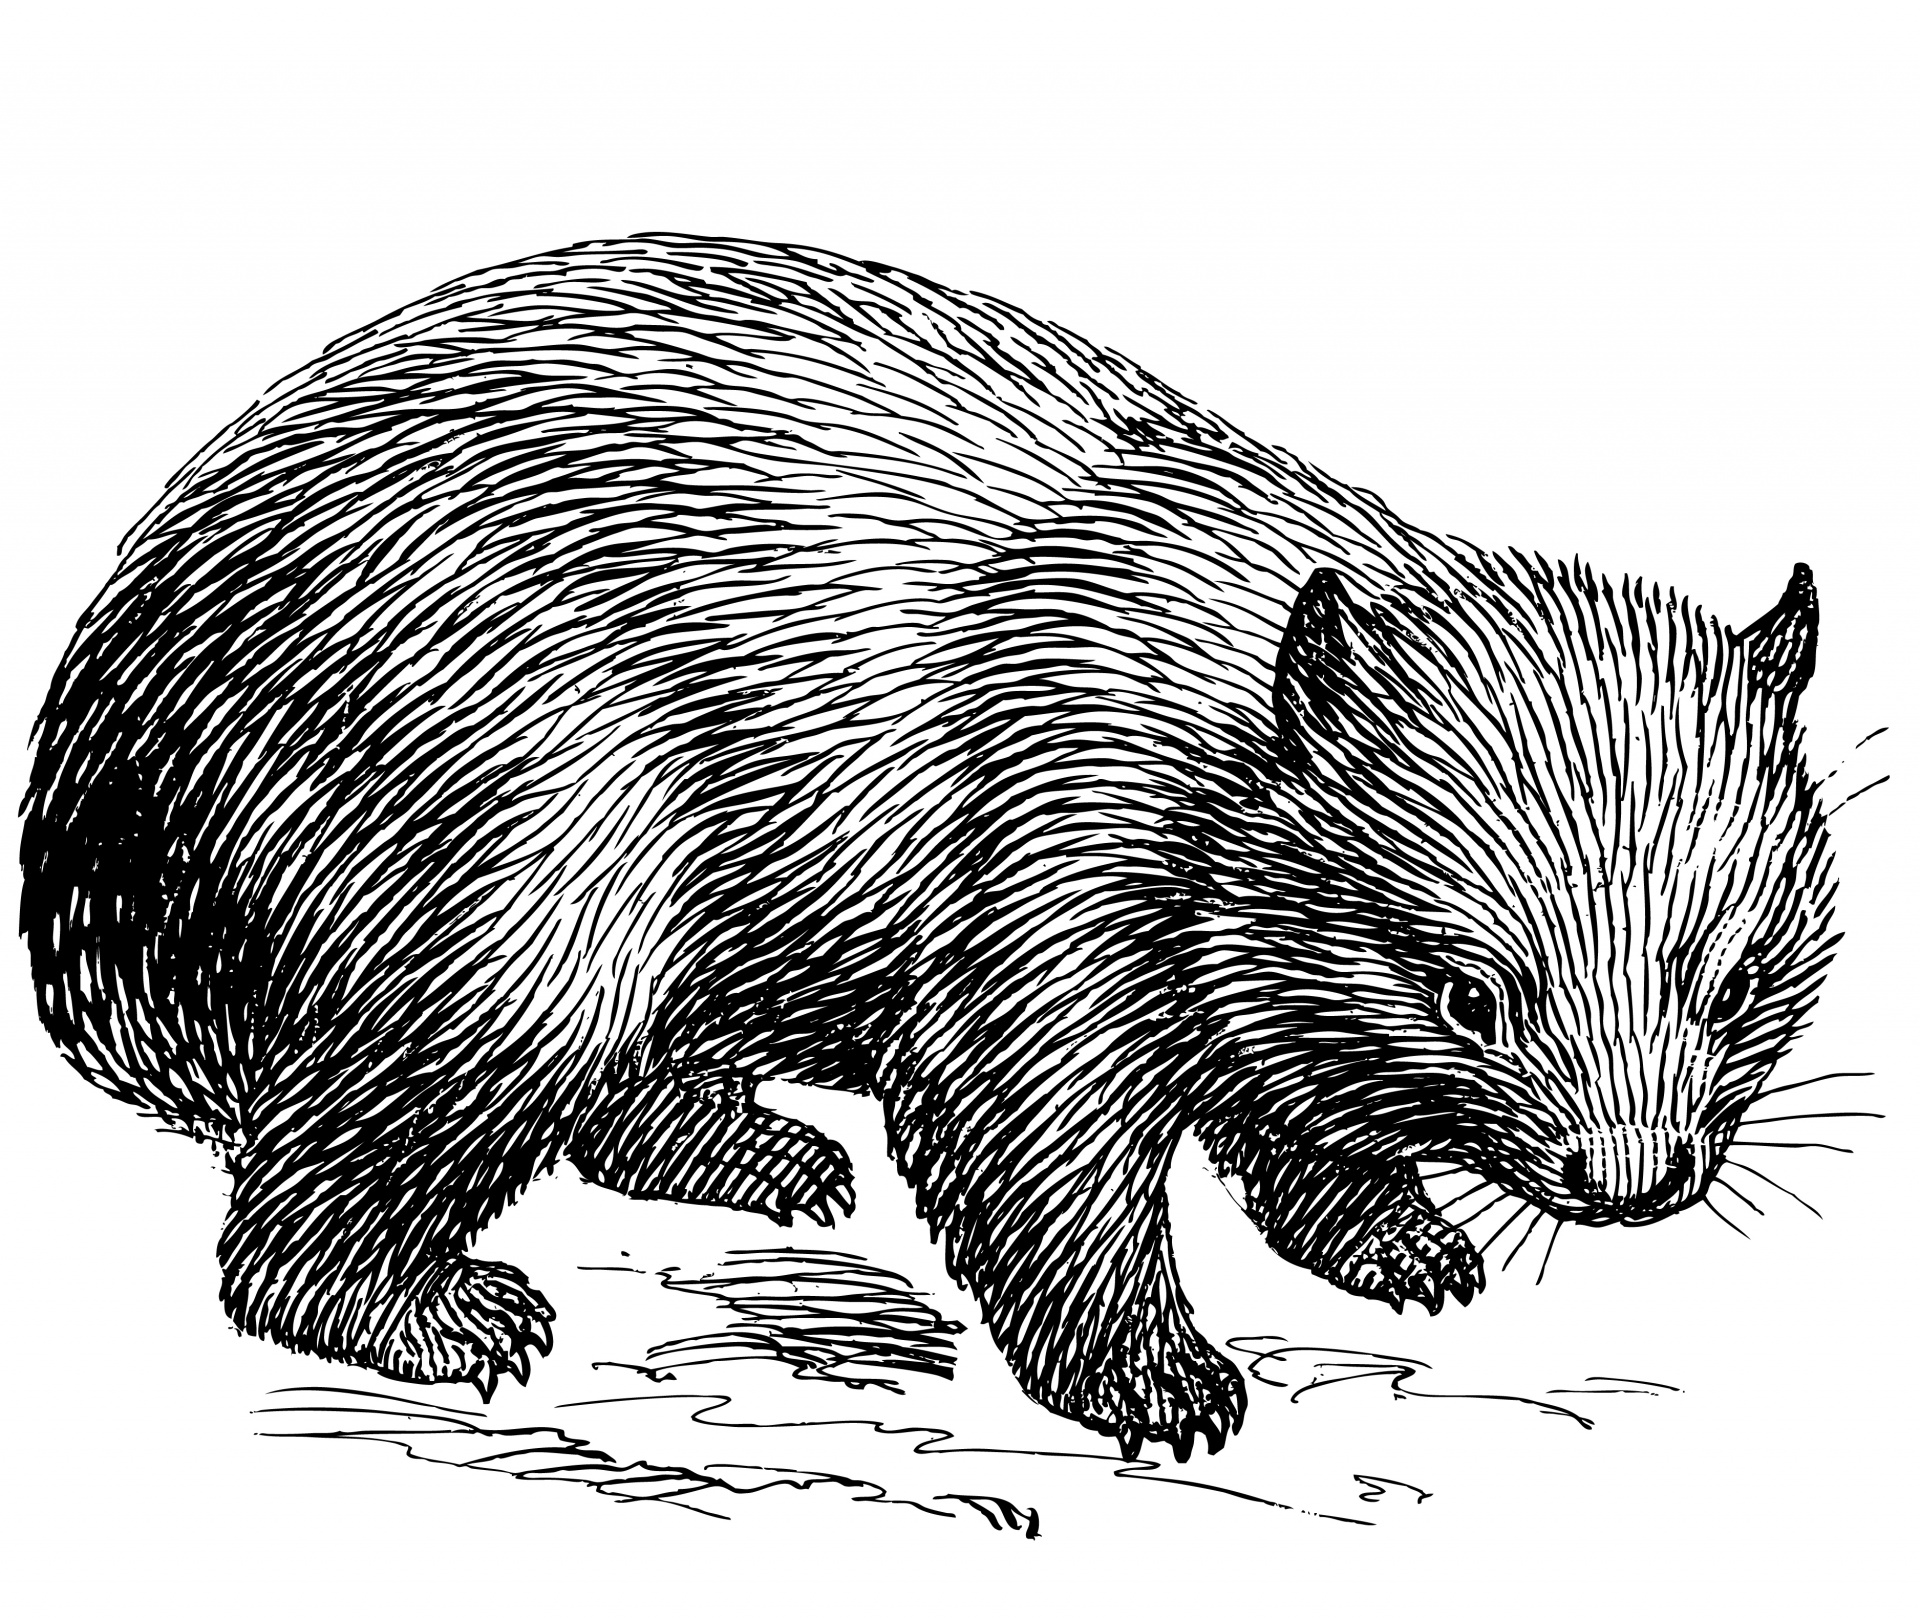
\includegraphics[height=4cm]{images/wombat} 
\end{center}

\item[Диджериду] Музыкальный инструмент австралийских аборигенов. Для примера, можно послушать ``David Hudson - Rainbow Serpent''. 

\item[``По теченью Пути''] Речь о нашей галактике -- Млечный Путь. Если посмотреть на ночное небо вдали от цивилизации и источников света, можно наблюдать что-то похожее на иллюстрацию на стр.~\pageref{milky-way} - боковой вид нашей галактики изнутри.

\item[Сверхнова] Сверхновая звезда -- заключающая фаза цикла жизни некоторых звёзд, в результате которой выделяется очень много энергии. Взрыв разбрасывает большое количество материи в пространство, при этом наблюдается очень яркая вспышка. Внимание, свехрновы лучше наблюдать издалека! Деструктивный потенциал этого явления может уничтожить любые формы жизни в отдельном регионе космоса. 


\item[Кинцуги] Японская традиция реставрации разбитой керамики. Мыцумото адепт этой идеи. Он считает что поломки и трещины -- часть жизни, и они составляют важную часть истории каждого из нас.

\item[Туар\'{е}ги] Кочевой народ проживающий на севере Африки, например в Алжире или Ливии. Традиционный наряд туарегов включает вещи цвета индиго (что-то между тёмно-синим и фиолетовым).


\item[Ф\'{е}нек] Маленькая лиса с большими ушами, обитает в пустынях на севере Африки. Имя происходит от арабского ``фанак'', что означает ``лиса''. 


\item[В\'{а}ди] В арабском языке, это русло высохшей реки. Иногда они могут временно заполняться после проливных дождей.
\end{description}



\subsection{Как распечатать эту книгу?}

\renewcommand{\thefootnote}{\fnsymbol{footnote}}

\begin{enumerate}
    \item Нужен принтер с опцией двусторонней печати.
    \item Открыть файл PDF в Adobe Acrobat Reader (именно в нём!).
    \item В меню \menu{Файл > Печать} (или \keys{\ctrl + P}) нажать на кнопку \menu{Booklet}.
    \item Согнуть\footnote[2]{Внимание! Вынимая бумагу из принтера, помни, что она может быть горячей! Настоятельно рекомендуется применение митрилловых перчаток!} страницы \emph{как есть}, они уже в нужном порядке.
    \item Закрепить степлером, вставить скобы вручную, или сшить.
\end{enumerate}


% this is the back-cover of the book
\cleartoverso
% \cleartoevenpage
% \clearpage
\thispagestyle{empty}  % to not have a page# here


\section*{Другие книги нашего издательства}
\vspace{2cm}

\begin{table}[h]
\begin{tabular}{ccc}
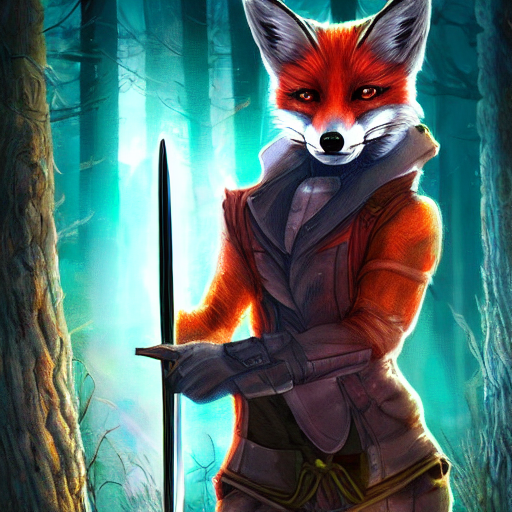
\includegraphics[height=5cm]{images/lisa-v-lesu} & 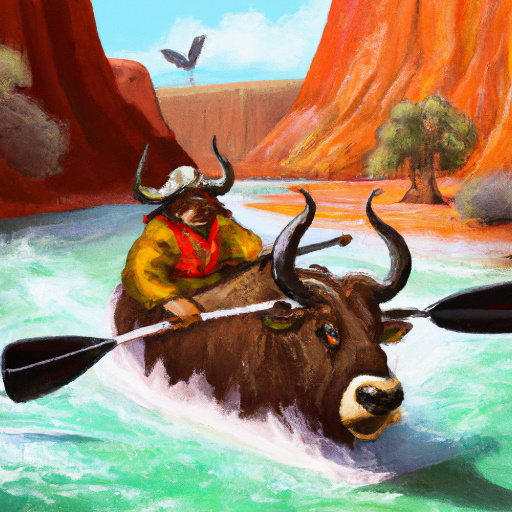
\includegraphics[height=5cm]{images/yak-kayak} & 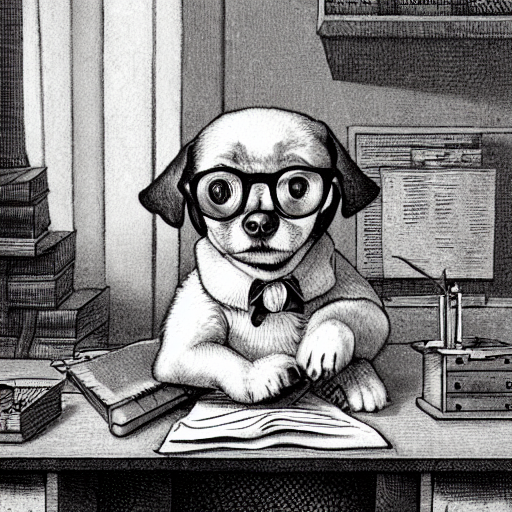
\includegraphics[height=5cm]{images/dog-book-cooker}             \\
 Лиса в лесу    &  Я, як, и каяк        &   Собака, которая            \\
  нашла косу &  & любила цифры \\
            &          &              \\
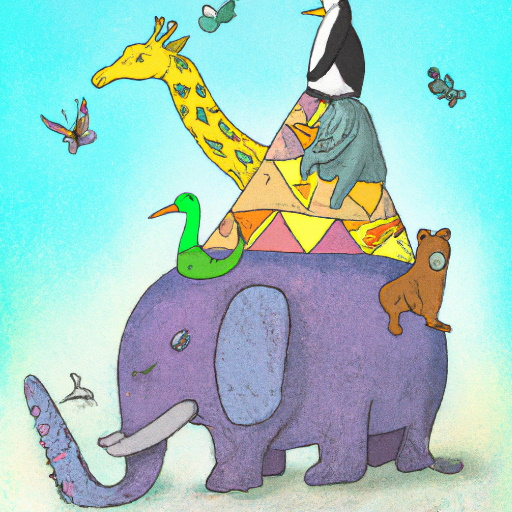
\includegraphics[height=5cm]{images/magic-pyramid} & 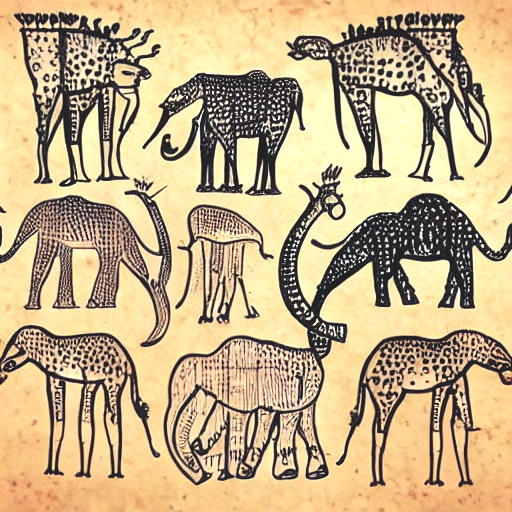
\includegraphics[height=5cm]{images/cave-stories} & 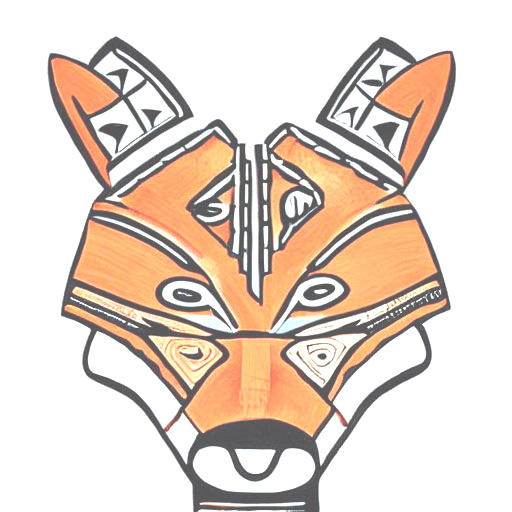
\includegraphics[height=5cm]{images/razukrashki.jpg}             \\
 На плечах гигантов       &  Волшебная пещера    &     Разукрашки \\    
        &      &     Дваукрашки \\
        &      &     Триукрашки \\
\end{tabular}
\end{table}


\end{document}


